%% =====================================================================
%%  M.Tech Project Report  -  Vadithe Sai Kumar Naik (CS25M053)
%%  PDDL-Based Mission Planning for a Drone Swarm Simulator
%%  Department of Computer Science and Engineering, IIT Madras
%%
%%  Report V4. Updated against the local plan files on 30 October 2026.
%%  Build:  pdflatex main.tex   (run twice so contents and lists update)
%%          or  tectonic main.tex
%%  Files:  figures/iitm_logo.png
%%          figures/screenshots/<plan>.png   (optional: simulator output
%%          screenshots; a placeholder box is drawn for any missing file,
%%          see figures/screenshots/README.txt for the expected names)
%% =====================================================================
\documentclass[11pt,a4paper,oneside]{report}

%% ---------- Personal details (edit here) ----------------------------
\newcommand{\thesistitle}{PDDL-Based Mission Planning for a Drone Swarm Simulator}
\newcommand{\thesistitlebreak}{PDDL-Based Mission Planning\\ for a Drone Swarm Simulator}
\newcommand{\authorname}{Vadithe Sai Kumar Naik}
\newcommand{\rollno}{CS25M053}
\newcommand{\submitdate}{December 2026}
\newcommand{\advisor}{Prof. N. S. Narayanaswamy}
\newcommand{\coadvisor}{Dr. Jaimandeep Singh}

%% ---------- Largest swarm each plan was planned for (edit here) -----
%% Measured through the real plan pipeline with the simulator's planning
%% time limit; used in the abstract and in the "at a glance" boxes.
\newcommand{\maxTravel}{60}
\newcommand{\maxSearch}{7}
\newcommand{\maxV}{9}
\newcommand{\maxGrid}{36}
\newcommand{\maxCube}{64}
\newcommand{\maxFig}{27}
\newcommand{\maxStar}{40}
\newcommand{\maxPlanets}{8}

%% ---------- Packages -------------------------------------------------
\usepackage{iftex}
\ifXeTeX
  \usepackage{newtxtext,newtxmath}
  \setmonofont[Scale=0.95,BoldFont=Inconsolatazi4-Bold.otf]{Inconsolatazi4-Regular.otf}
\else
  \usepackage[T1]{fontenc}
  \usepackage[utf8]{inputenc}
  \usepackage{newtxtext,newtxmath}
  \usepackage[varqu,scaled=0.95]{zi4}
\fi
\usepackage[a4paper,top=1in,bottom=1in,left=1.2in,right=1in]{geometry}
\usepackage{setspace}
\setstretch{1.3}
\usepackage{graphicx}
\usepackage{booktabs,tabularx,array,multirow,longtable}
\newcolumntype{Y}{>{\raggedright\arraybackslash}X}
\newcolumntype{P}[1]{>{\raggedright\arraybackslash}p{#1}}
\usepackage{enumitem}
\setlist{itemsep=2pt,topsep=4pt}
\usepackage[table]{xcolor}
\usepackage{amsmath}
\usepackage{listings}
\usepackage{tikz}
\usetikzlibrary{arrows.meta,positioning,shapes.geometric,shapes.misc,fit,calc,backgrounds,decorations.pathreplacing}
\usepackage{pgfplots}
\pgfplotsset{compat=1.17}
\usepackage[most]{tcolorbox}
\usepackage{needspace}
\usepackage[font=small,labelfont=bf,labelsep=colon]{caption}
\captionsetup[table]{justification=raggedright,singlelinecheck=false,skip=6pt}
\captionsetup[figure]{format=hang,skip=6pt}
\usepackage{titlesec}
\usepackage{titletoc}
\usepackage{float}
\usepackage{xurl}
\usepackage[hidelinks]{hyperref}
\hypersetup{
  pdftitle={\thesistitle},
  pdfauthor={\authorname},
  pdfsubject={M.Tech thesis, IIT Madras}
}

% Never leave a single line of a paragraph alone at the top or bottom of a page
\widowpenalty=10000
\clubpenalty=10000
\displaywidowpenalty=10000
% Allow a little extra word spacing rather than letting long code words run into the margin
\setlength{\emergencystretch}{3em}

%% ---------- Colours --------------------------------------------------
\definecolor{navy}{HTML}{0F2240}
\definecolor{amber}{HTML}{F0A30A}
\definecolor{codebg}{HTML}{F5F5F5}
\definecolor{coderule}{HTML}{C8C8C8}
\definecolor{kwblue}{HTML}{1F5FBF}
\definecolor{cmtgray}{HTML}{7A7A7A}
\definecolor{okgreen}{HTML}{2E7D32}
\definecolor{warnred}{HTML}{C62828}
\definecolor{softblue}{HTML}{E8EEF7}
\definecolor{softamber}{HTML}{FDF1D8}

%% ---------- Chapter and section headings ----------------------------
\titleformat{\chapter}[display]
  {\centering\bfseries}
  {\LARGE\chaptertitlename\ \thechapter}
  {1.6em}
  {\huge}
\titlespacing*{\chapter}{0pt}{10pt}{28pt}
\titleformat{name=\chapter,numberless}[block]
  {\centering\bfseries\huge}{}{0pt}{}
\titlespacing*{name=\chapter,numberless}{0pt}{10pt}{24pt}
\titleformat{\section}{\bfseries\Large}{\thesection}{0.6em}{}
\titleformat{\subsection}{\bfseries\large}{\thesubsection}{0.6em}{}
\titleformat{\paragraph}[runin]{\bfseries}{}{0pt}{}[.]
\titlespacing*{\section}{0pt}{20pt}{10pt}
\titlespacing*{\subsection}{0pt}{14pt}{6pt}
\titlespacing*{\paragraph}{0pt}{10pt}{0.6em}
\setcounter{secnumdepth}{3}
\setcounter{tocdepth}{1}

%% ---------- Contents, list of tables, list of figures ---------------
%% All entries share one left edge and one gap, so that front matter,
%% chapters and references line up in the contents.
\renewcommand{\contentsname}{Contents}
\renewcommand{\listtablename}{List of Tables}
\renewcommand{\listfigurename}{List of Figures}
\newlength{\tocgap}\setlength{\tocgap}{1.0em}
\titlecontents{chapter}[0pt]
  {\addvspace{\tocgap}\bfseries}
  {\makebox[7.2em][l]{CHAPTER \thecontentslabel}\MakeUppercase}
  {\MakeUppercase}
  {\hfill\contentspage}
  []
\titlecontents{section}[7.2em]
  {\addvspace{0.2em}\small}
  {\contentslabel{3.0em}}
  {}
  {\titlerule*[0.7pc]{.}\contentspage}
\titlecontents{figure}[4.2em]
  {\vspace{0.4em}\small}
  {\hspace*{-4.2em}\makebox[4.2em][l]{\thecontentslabel}}
  {}
  {\titlerule*[0.7pc]{.}\contentspage}
\titlecontents{table}[4.2em]
  {\vspace{0.4em}\small}
  {\hspace*{-4.2em}\makebox[4.2em][l]{\thecontentslabel}}
  {}
  {\titlerule*[0.7pc]{.}\contentspage}
% Front-matter entries in the contents (bold, upper case, no dots)
\newcommand{\frontentry}[2]{\addvspace{\tocgap}\noindent\textbf{#1}\hfill\textbf{#2}\par}
\newcommand{\addfront}[1]{\addtocontents{toc}{\protect\frontentry{#1}{\thepage}}}
% The report class adds an extra gap to the lists at every new chapter;
% switch it off so that every entry is spaced the same way.
\makeatletter
\newcommand{\nochaptergap}{\let\addvspace\@gobble}
\makeatother

%% ---------- Code listings (PDDL) -------------------------------------
\lstdefinelanguage{PDDL}{
  morekeywords=[1]{define,domain,problem,and,or,not,forall,exists,when,imply,
    increase,decrease,assign,either},
  morekeywords=[2]{:requirements,:types,:predicates,:functions,:action,
    :parameters,:precondition,:effect,:objects,:init,:goal,:domain,:strips,
    :typing,:numeric-fluents,:negative-preconditions,:conditional-effects,
    :equality,:disjunctive-preconditions,:universal-preconditions},
  sensitive=false,
  morecomment=[l]{;},
  alsoletter={:-},
}
\lstset{
  language=PDDL,
  basicstyle=\ttfamily\footnotesize\setstretch{1.0},
  keywordstyle=[1]\color{kwblue}\bfseries,
  keywordstyle=[2]\color{kwblue},
  commentstyle=\color{cmtgray}\itshape,
  backgroundcolor=\color{codebg},
  frame=single,
  rulecolor=\color{coderule},
  framesep=4pt,
  xleftmargin=6pt,xrightmargin=6pt,
  aboveskip=8pt,belowskip=8pt,
  breaklines=true,
  breakatwhitespace=true,
  columns=fullflexible,
  keepspaces=true,
  showstringspaces=false,
  tabsize=4,
}
\lstdefinestyle{plain}{language={},keywordstyle=,commentstyle=}

\newcommand{\code}[1]{\texttt{#1}}
\newcommand{\recordlabel}[1]{\par\smallskip\noindent\hspace*{1.2em}\textit{#1}\par}

%% ---------- "At a glance" box for each plan --------------------------
\newcommand{\glancebox}[2]{%
  \begin{tcolorbox}[enhanced,colback=softblue!45,colframe=navy,coltitle=white,
      fonttitle=\bfseries\small,title={#1},boxrule=0.6pt,arc=2pt,
      left=6pt,right=6pt,top=3pt,bottom=3pt,before skip=8pt,after skip=10pt]
    \small\setstretch{1.1}%
    \begin{tabularx}{\linewidth}{@{}>{\bfseries}P{0.25\linewidth}Y@{}}#2\end{tabularx}
  \end{tcolorbox}}

%% ---------- Action order strip ----------------------------------------
\newcommand{\then}{\,{\color{amber!80!black}$\boldsymbol{\rightarrow}$}\allowbreak\,}
\newcommand{\actionflow}[1]{%
  \par\begin{tcolorbox}[colback=codebg,colframe=coderule,boxrule=0.4pt,arc=2pt,
      left=5pt,right=5pt,top=2pt,bottom=2pt,before skip=6pt,after skip=8pt]
    \footnotesize\ttfamily\raggedright\setstretch{1.25}#1
  \end{tcolorbox}}

%% ---------- Screenshot of a plan's output (placeholder if missing) ---
%% #1 file name in figures/screenshots, #2 short caption, #3 caption, #4 label
\newcommand{\screenshot}[4]{%
  \begin{figure}[H]
  \centering
  \IfFileExists{figures/screenshots/#1}{%
    \includegraphics[width=0.92\textwidth]{figures/screenshots/#1}}{%
    \begin{tikzpicture}
      \draw[navy!60,dashed,line width=0.9pt,fill=softblue!35,rounded corners=4pt]
        (0,0) rectangle (12.5,5.0);
      \node[align=center,font=\small,text=navy] at (6.25,2.5)
        {\textbf{Simulator output for this plan}\\[4pt]
         Screenshot to be added: \texttt{figures/screenshots/#1}};
    \end{tikzpicture}}
  \caption[#2]{#3}
  \label{#4}
  \end{figure}}

%% ---------- Reusable TikZ styles -------------------------------------
\tikzset{
  drone/.style={circle,fill=navy,minimum size=7pt,inner sep=0pt},
  leader/.style={circle,fill=amber,minimum size=9pt,inner sep=0pt},
  link/.style={navy,line width=0.7pt},
  box/.style={draw=navy,line width=0.8pt,rounded corners=3pt,fill=softblue,
              align=center,font=\small,inner sep=5pt,minimum height=2.2em},
  abox/.style={box,fill=softamber,draw=amber!80!black},
  gbox/.style={box,fill=white},
  arr/.style={-{Stealth[length=5pt]},line width=0.8pt,navy},
  darr/.style={arr,dashed},
  % communication diagrams
  focus/.style={circle,fill=warnred,minimum size=10pt,inner sep=0pt},
  nbr/.style={circle,fill=navy,draw=amber,line width=1.3pt,minimum size=9pt,inner sep=0pt},
  other/.style={circle,fill=gray!45,minimum size=7pt,inner sep=0pt},
  comm/.style={{Stealth[length=4pt]}-{Stealth[length=4pt]},okgreen!70!black,line width=1pt},
  commthin/.style={okgreen!60!black,line width=0.45pt},
  gcs/.style={rectangle,draw=navy,fill=softamber,rounded corners=2pt,
              font=\scriptsize\bfseries,inner sep=3pt},
  glink/.style={{Stealth[length=3.5pt]}-{Stealth[length=3.5pt]},navy!60,dashed,line width=0.6pt},
  note/.style={font=\scriptsize,align=left,text width=4.3cm},
  cnt/.style={font=\tiny\bfseries,text=warnred},
}

\begin{document}

%% =====================================================================
%%  COVER PAGE
%% =====================================================================
\begin{titlepage}
\thispagestyle{empty}
\noindent
\begin{minipage}[c]{0.36\textwidth}
  
\includegraphics[width=0.62\linewidth]{figures/iitm_logo.png}
\end{minipage}%
\begin{minipage}[c]{0.64\textwidth}
  \setstretch{1.05}\small
  DEPARTMENT OF COMPUTER SCIENCE AND\\
  ENGINEERING\\
  INDIAN INSTITUTE OF TECHNOLOGY MADRAS\\
  CHENNAI -- 600036
\end{minipage}

\vspace{0.6cm}
\noindent\rule{\textwidth}{2pt}

\vspace{2.0cm}
\begin{center}
  {\setstretch{1.2}\LARGE\bfseries \thesistitlebreak\par}

  \vspace{1.4cm}
  % ---- Emblem: PDDL model -> planner -> plan -> swarm flight ----
  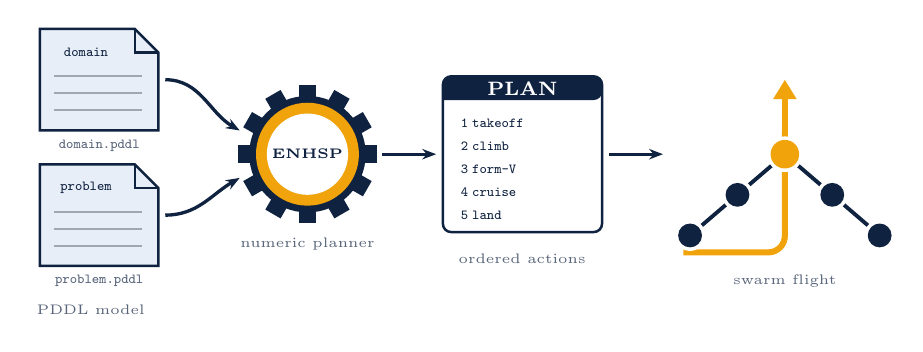
\begin{tikzpicture}[scale=0.86,every node/.style={font=\scriptsize}]
    % two PDDL files
    \foreach \y/\name in {0.35/domain,-1.65/problem} {
      \begin{scope}[shift={(-6.4,\y)}]
        \filldraw[fill=softblue,draw=navy,line width=0.9pt]
          (0,0)--(1.75,0)--(1.75,1.15)--(1.4,1.5)--(0,1.5)--cycle;
        \draw[navy,line width=0.9pt] (1.4,1.5)--(1.4,1.15)--(1.75,1.15);
        \foreach \l in {0.3,0.55,0.8} \draw[navy!40,line width=0.8pt] (0.2,\l)--(1.5,\l);
        \node[font=\tiny\bfseries\ttfamily,text=navy] at (0.68,1.15) {\name};
        \node[font=\tiny\ttfamily,text=navy!70] at (0.875,-0.22) {\name.pddl};
      \end{scope}
    }
    \draw[arr,line width=1.2pt] (-4.55,1.1) to[out=0,in=150] (-3.45,0.35);
    \draw[arr,line width=1.2pt] (-4.55,-0.9) to[out=0,in=-150] (-3.45,-0.35);
    % planner gear
    \begin{scope}[shift={(-2.45,0)}]
      \foreach \a in {0,30,...,330}
        \fill[navy,rotate=\a] (0.78,-0.13) rectangle (1.02,0.13);
      \fill[navy] (0,0) circle (0.86);
      \fill[amber] (0,0) circle (0.76);
      \fill[white] (0,0) circle (0.6);
      \node[font=\tiny\bfseries,text=navy] at (0,0) {ENHSP};
      \node[font=\tiny,text=navy!70] at (0,-1.32) {numeric planner};
    \end{scope}
    \draw[arr,line width=1.2pt] (-1.35,0)--(-0.55,0);
    % plan
    \begin{scope}[shift={(-0.45,-1.15)}]
      \filldraw[fill=white,draw=navy,line width=0.9pt,rounded corners=3pt] (0,0) rectangle (2.35,2.3);
      \fill[navy] (0,1.95) [rounded corners=3pt] -- (0,2.3) -- (2.35,2.3) -- (2.35,1.95) [sharp corners] -- cycle;
      \node[font=\scriptsize\bfseries,text=white] at (1.175,2.12) {PLAN};
      \foreach \i/\t in {1/takeoff,2/climb,3/form-V,4/cruise,5/land}
        \node[anchor=west,font=\tiny\ttfamily,text=navy] at (0.12,1.95-\i*0.34) {\i\;\t};
    \end{scope}
    \draw[arr,line width=1.2pt] (2.0,0)--(2.8,0);
    % swarm flying the plan
    \begin{scope}[shift={(4.6,-0.55)}]
      \draw[amber,line width=2.2pt,rounded corners=6pt] (-1.5,-0.9)--(0,-0.9)--(0,0.9);
      \draw[amber,line width=2.2pt,-{Triangle[length=7pt,width=8pt]}] (0,0.8)--(0,1.65);
      \coordinate (L) at (0,0.55);
      \coordinate (A1) at (-0.7,-0.05); \coordinate (A2) at (-1.4,-0.65);
      \coordinate (B1) at (0.7,-0.05);  \coordinate (B2) at (1.4,-0.65);
      \draw[navy,line width=1.4pt] (A2)--(A1)--(L)--(B1)--(B2);
      \foreach \p in {A1,A2,B1,B2} {\fill[white] (\p) circle (6.5pt); \fill[navy] (\p) circle (5pt);}
      \fill[white] (L) circle (7.5pt); \fill[amber] (L) circle (6pt);
      \node[font=\tiny,text=navy!70] at (0,-1.32) {swarm flight};
    \end{scope}
    \node[font=\tiny,text=navy!70] at (-5.65,-2.3) {PDDL model};
    \node[font=\tiny,text=navy!70] at (0.72,-1.55) {ordered actions};
  \end{tikzpicture}

  \vspace{1.6cm}
  {\itshape A Thesis\par}
  \vspace{0.25cm}
  {\itshape Submitted by\par}
  \vspace{0.3cm}
  {\Large\bfseries \authorname\par}
  \vspace{1.0cm}
  {\itshape For the award of the degree\par}
  \vspace{0.25cm}
  {\itshape Of\par}
  \vspace{0.25cm}
  {\bfseries MASTER OF TECHNOLOGY\par}
  \vspace{0.2cm}
  \submitdate
\end{center}
\end{titlepage}

%% =====================================================================
%%  THESIS CERTIFICATE
%% =====================================================================
\thispagestyle{empty}
\begin{center}
  {\LARGE\bfseries Thesis Certificate\par}
\end{center}
\vspace{0.8cm}
\noindent This is to certify that the thesis entitled \textbf{\thesistitle}, submitted by
\textbf{\authorname\ (\rollno)} to the Indian Institute of Technology Madras in partial
fulfilment of the requirements for the degree of \textbf{Master of Technology}, is a bona fide
record of the work carried out under the guidance of \textbf{\advisor}, Project Advisor, and
\textbf{\coadvisor}, Project Co-Advisor.

\noindent The contents of this thesis, in full or in part, have not been submitted to any other
institute or university for the award of a degree or diploma.

\vspace{2.2cm}
\noindent
\begin{minipage}[t]{0.5\textwidth}
  \setstretch{1.15}
  Chennai 600036\\
  Date: \submitdate
\end{minipage}%
\begin{minipage}[t]{0.5\textwidth}
  \raggedleft\setstretch{1.15}
  \textbf{\authorname}\\
  \rollno
\end{minipage}

\vspace{2.6cm}
\begin{flushright}
  \setstretch{1.15}
  \textbf{\advisor}\\
  Project Advisor, Professor\\
  Department of Computer Science and Engineering\\
  Indian Institute of Technology Madras
\end{flushright}

\vspace{1.8cm}
\begin{flushright}
  \setstretch{1.15}
  \textbf{\coadvisor}\\
  Project Co-Advisor\\
  Department of Computer Science and Engineering\\
  Indian Institute of Technology Madras
\end{flushright}

\vfill
\noindent{\small \textcopyright\ 2026 Indian Institute of Technology Madras}
\clearpage

%% =====================================================================
%%  FRONT MATTER
%% =====================================================================
\pagenumbering{roman}
\pagestyle{plain}

\addtocontents{toc}{\protect\noindent\protect\hfill\protect\textbf{Page}\protect\par}
\addtocontents{lot}{\protect\nochaptergap\protect\small\protect\noindent\protect\makebox[4.2em][l]{\protect\textbf{Table}}\protect\textbf{Caption}\protect\hfill\protect\textbf{Page}\protect\par\protect\vspace{0.5em}}
\addtocontents{lof}{\protect\nochaptergap\protect\small\protect\noindent\protect\makebox[4.2em][l]{\protect\textbf{Figure}}\protect\textbf{Caption}\protect\hfill\protect\textbf{Page}\protect\par\protect\vspace{0.5em}}

\chapter*{Acknowledgements}
\addfront{ACKNOWLEDGEMENTS}
I would like to express my sincere gratitude to my project guide \textbf{\advisor} for his
exceptional guidance, unwavering support, and encouragement throughout this project. His insights
and constructive feedback were instrumental in shaping the direction of this work and continually
motivated me to improve its quality.

I am also grateful to my co-guide \textbf{\coadvisor} for his invaluable support and assistance.
His technical insights and thoughtful suggestions broadened my perspective and significantly
enhanced the outcome of this project.

Furthermore, I would like to thank the faculty and staff of the Department of Computer Science
and Engineering, IIT Madras, for providing the resources and environment necessary for carrying
out this work.

\chapter*{Abstract}
\addfront{ABSTRACT}
\noindent\textbf{Keywords:} automated planning; PDDL; numeric planning; ENHSP; drone swarm;
formation flight; fault handling; battery management.

\medskip
A drone swarm mission is more than a route. Before a drone may take off, join a formation or
continue a leg, its battery must cover the next move, its GPS and radio links must work, its
health must be acceptable and its neighbours in the formation must be in place. This thesis
describes the planning layer of a drone swarm simulator, in which these rules are written in the
Planning Domain Definition Language (PDDL) and solved by the Expressive Numeric Heuristic Search
Planner (ENHSP). In this work I designed and built this complete PDDL planning layer.

Fourteen simulator mission plans were developed, each as a domain file and a problem template: point-to-point
travel, forest area search, V formation, two-dimensional grid formation, three-dimensional
(cube) grid formation, parabola formation, figure-eight train formation, star drone show,
planetary orbit show, road inspection, battery-aware travel, Formula-4 and a rotating circle.
Task allocation lets a standby drone take over after an active drone reports a problem.
The original plans share a vocabulary of drone states,
health flags, failure states and numeric fluents for battery, energy, altitude and health. A
plan service retargets each template onto the points the operator picks on the map, expands it
to the number of selected drones and passes it to ENHSP. Only the leader corridor is usually
planned symbolically; the other drones' routes are then derived geometrically from their
formation slots.

Battery-aware travel adds charging stops with a next-hop charge target. Formula-4 and the
rotating circle change positions and heights using one shared clock, without exchanging
neighbour positions. Task allocation also has a runtime controller for launching a standby and transferring task data.

Inter-drone communication in the original formations is modelled in two layers. In PDDL, each formation declares which
drones are neighbours and every formation action checks a per-drone \code{neighbor-comm-ok}
flag; the parabola plan goes further and requires each directed link to be established within
a communication range. At run time the ground station talks to each drone over a JSON-over-UDP
protocol with heartbeats, and formation keeping for trains and shows runs on board each drone
against a shared, time-stamped pace. Four fault types are modelled in the domains -- GPS loss,
communication loss, neighbour-link loss and health failure -- together with ground-controller
responses such as return, hover and sacrifice. Battery health is handled both as a planning
resource and at run time through low and critical thresholds that pause the swarm and ask the
operator to decide.

The original swarm templates support a selected number of drones within their limits.
Formula-4 and Formation-Circle use four drones, battery-aware travel uses one, and the separate
task-allocation plan uses four candidates. Within the simulator's
planning time limit, point-to-point travel adapts to as many as \maxTravel{} drones, forest
search to \maxSearch{}, the V formation to \maxV{} (odd counts), the two-dimensional grid to
\maxGrid{} and the cube formation to \maxCube{} drones. The figure-eight train adapts up to the
capacity of the eight the operator draws (\maxFig{} drones on a typical eight), the star show to
6--\maxStar{} drones and the planetary show to 2--\maxPlanets{} drones, while the parabola uses
exactly three drones and road inspection one. The report also records the modelling lessons
learnt during verification and the limits of the present approach.

\clearpage
\addfront{CONTENTS}
\tableofcontents
\clearpage
\addfront{LIST OF TABLES}
\listoftables
\clearpage
\addfront{LIST OF FIGURES}
\listoffigures

\chapter*{Abbreviations}
\addfront{ABBREVIATIONS}
\begin{center}
\begin{tabular}{@{}p{0.22\textwidth}p{0.68\textwidth}@{}}
\toprule
\textbf{Abbreviation} & \textbf{Meaning} \\
\midrule
PDDL   & Planning Domain Definition Language \\
ENHSP  & Expressive Numeric Heuristic Search Planner \\
GCS    & Ground Control Station \\
GUI    & Graphical User Interface \\
UAV    & Unmanned Aerial Vehicle \\
SYSID  & MAVLink system identifier of a drone \\
MAVLink& Micro Air Vehicle Link, a lightweight drone messaging protocol \\
UDP    & User Datagram Protocol \\
JSON   & JavaScript Object Notation \\
OSRM   & Open Source Routing Machine \\
AIBR   & Additive Interval Based Relaxation (ENHSP preprocessing) \\
RTL    & Return to Launch \\
\bottomrule
\end{tabular}
\end{center}

\clearpage
\pagenumbering{arabic}

%% =====================================================================
%%  CHAPTER 1  INTRODUCTION
%% =====================================================================
\chapter{Introduction}

\section{Background and Motivation}
Small unmanned aerial vehicles are now used for search, inspection, mapping and public light
shows. Many of these tasks are done better by a group of drones than by one drone. A group,
however, needs coordination. Each drone must know when to take off, which place in the
formation it must hold, which other drones it must stay in contact with, and what to do when
something goes wrong. Writing these rules directly in flight code makes them hard to read, hard
to check and hard to change.

Automated planning offers a cleaner way. In planning, the rules of the world are written once as
a \emph{domain}: a set of actions, each with the conditions under which it may be applied and the
changes it causes. A particular mission is written as a \emph{problem}: the drones, the places,
the starting state and the goal. A general-purpose planner then searches for a sequence of
actions that reaches the goal while respecting every rule. PDDL is the standard language for
writing such domains and problems.

This project is part of a larger drone swarm simulator built in the department. The simulator
runs each drone as an independent thread and offers a ground station GUI with a map, telemetry
and fault injection. The work reported here is the planning layer of that simulator: the PDDL
models for every mission type, and their link to the rest of the system.

\section{Problem Statement and Objectives}
The central problem is to express swarm missions -- including formations, communication
requirements, battery limits and failures -- in PDDL in a way that a numeric planner can solve
quickly for realistic swarm sizes, and whose plans can be turned into flyable routes. The work
had the following objectives:
\begin{enumerate}
  \item Design a common PDDL vocabulary for drone state, health, communication, battery and
        failure that every mission plan can share.
  \item Build domain and problem files for a range of missions: travel, area search, rigid
        formations (V, grid, cube, parabola), path-following trains (figure-eight), shape-changing
        shows (star, planets) and road inspection.
  \item Model drone-to-drone communication, so that a formation can only form and fly while the
        required links are up.
  \item Model faults (GPS, communication, neighbour link, health) and battery health, together
        with the ground controller's responses.
  \item Integrate the plans with the simulator, so that a plan is retargeted to the operator's map
        inputs, solved by ENHSP and executed by the drones, and verify the results.
\end{enumerate}

\section{Scope and Contributions}
My main contribution in this work is the complete PDDL planning layer of the simulator. In
particular, this work contributes:
\begin{itemize}
  \item fourteen simulator mission plans (Table~\ref{tab:inventory}) including task allocation, using shared names where the same idea applies; the original
        swarm templates adapt
        to the number of drones the operator selects;
  \item a set of modelling patterns that keep formation problems tractable for large swarms:
        planning only the leader corridor, descriptive neighbour relations with per-drone
        communication flags, and propositional rather than numeric gates for ordered launches;
  \item a two-level model of communication: symbolic neighbour links in PDDL, including an
        explicit range-checked link model in the parabola plan, and the run-time protocol used
        by the ground station and the drones;
  \item a fault and battery model covering four failure types, ground-controller responses and
        energy accounting for travel, climb, cruise and hover;
  \item verification of the simulator plans through the real planning pipeline, including scalability
        measurements and a record of the modelling defects found and fixed.
\end{itemize}

Besides the planning layer, I also worked on parts of the ground station GUI, in particular the
mission planner panel through which the operator chooses a plan and picks its points on the map.
The remaining parts of the simulator, such as the MAVLink message conversion and the flight
firmware emulation, were developed by other members of the project team. This thesis therefore
focuses on PDDL-based planning; the other parts are described only as far as needed to explain
how a PDDL plan becomes a flight. All results in this report come from the simulator.

\section{Organisation of the Report}
Chapter~\ref{ch:background} reviews automated planning, PDDL, numeric planning and related work
on multi-drone missions. Chapter~\ref{ch:arch} explains the simulator architecture and the
planning pipeline step by step. Chapter~\ref{ch:model} presents the common PDDL vocabulary and
design patterns. Chapter~\ref{ch:plans} explains the mission plans one by one: what each
mission does, how its drones communicate, the important parts of its PDDL and its output.
Chapter~\ref{ch:comm} explains how drones communicate, both in the model and at run time.
Chapter~\ref{ch:faults} covers faults and battery health. Chapter~\ref{ch:results} reports the
verification results and the defects found. Chapter~\ref{ch:discussion} discusses limitations,
and Chapter~\ref{ch:conclusion} concludes with future work.

%% =====================================================================
%%  CHAPTER 2  BACKGROUND AND LITERATURE REVIEW
%% =====================================================================
\chapter{Background and Literature Review}\label{ch:background}

\section{Automated Planning}
Classical planning studies how an agent can reach a goal from a known initial state by applying
actions with known effects. A planning task is described by a set of state variables, a set of
actions and a goal. Each action has a \emph{precondition} that must hold before it is applied
and an \emph{effect} that changes the state. A \emph{plan} is a sequence of actions that, applied
in order from the initial state, ends in a state that satisfies the goal. Heuristic search
planners find such plans by estimating, for each state, how far it is from the goal and
expanding the most promising states first.

\section{The Planning Domain Definition Language}
PDDL was introduced to give planning competitions a common input language. A PDDL model is
split into two files:
\begin{itemize}
  \item the \textbf{domain} defines object types, \emph{predicates} (true/false facts such as
        \code{(gps-ok ?d)}), \emph{functions} (numeric values such as \code{(battery ?d)}) and
        \emph{actions};
  \item the \textbf{problem} names the concrete objects, gives the initial facts and values, and
        states the goal.
\end{itemize}

\noindent PDDL\,2.1 added \emph{numeric fluents}, so that actions can test and change numbers.
For example, a move can require enough charge and then use it up:

\begin{lstlisting}
:precondition (> (battery ?d) (energy-required ?from ?to))
:effect       (decrease (battery ?d) (energy-required ?from ?to))
\end{lstlisting}

\noindent Later PDDL versions added further requirements. The three used most in this work are:
\begin{itemize}
  \item \code{:universal-preconditions} -- a condition over every object of a type, for example
        ``\emph{every} wing drone is in its slot'';
  \item \code{:conditional-effects} -- an effect that applies only to some objects, for example
        ``move each drone \emph{that is} a wing drone'';
  \item \code{:negative-preconditions} -- a condition that a fact is \emph{false}, for example
        ``only if this drone is \emph{not} already in formation''.
\end{itemize}

\section{Numeric Planning with ENHSP}
ENHSP is a heuristic search planner for PDDL\,2.1 problems with numeric fluents. It grounds the
domain into concrete actions, runs a relaxation-based preprocessing step (AIBR) that also
detects some unsolvable problems early, and then searches with numeric heuristics. Two
properties of ENHSP mattered in this project. First, its heuristics estimate progress well for
conditions that compare a fluent with a constant, but poorly for conditions that compare two
fluents with each other. Second, its grounding step can use a large amount of memory for domains
with many drones and quantified conditions; a ``naive'' grounder option (\code{-gro naive}) helps
for formation domains. Both points shaped the models in Chapter~\ref{ch:model}.

\section{Multi-Drone Missions and Formations}
Aerial swarm research covers formation control, task allocation and collective behaviour.
Formation flight is often treated with a leader--follower scheme, in which one drone follows the
planned path and the others hold an offset from it. Early work on flocking showed that simple
local rules with near neighbours are enough for coherent group motion. This project borrows both
ideas: the planner reasons about a leader corridor, and each drone is required to stay in contact
only with its immediate neighbours. For curved paths, shortest paths with a bounded turning
radius are known as Dubins paths, and such paths are used to join the figure-eight pattern
smoothly.

\section{Fault-Aware Planning for UAVs}
Real drones lose GPS, lose radio contact and run out of battery. A plan that ignores these events
is not safe to fly. In planning, faults are commonly handled either by monitoring execution and
replanning, or by including recovery actions in the domain. This work follows the second idea in
a light form: each domain includes detection actions that turn a failed health flag into a failure
state and a controller notification, and the point-to-point domain adds explicit controller
orders (return, hover, sacrifice). Battery is treated as a numeric resource, so that the planner
itself refuses any move the drone cannot afford.

\section{Position of This Work}
The contribution is not a new planning algorithm. It is a family of carefully engineered PDDL
models for drone swarm missions, connected to a working simulator, together with an honest record
of what the models express, how they scale and where they stop. The models are written to be
read by people as well as solved by a planner, so that a supervisor or teammate can check every
safety rule directly in the PDDL.

%% =====================================================================
%%  CHAPTER 3  SYSTEM ARCHITECTURE
%% =====================================================================
\chapter{System Architecture and Planning Pipeline}\label{ch:arch}

\section{Simulator Overview}
The simulator has four main parts. The \textbf{ground station GUI} (PySide6) shows the map,
telemetry, the mission planner panel and fault injection controls. The \textbf{plan service}
prepares PDDL problems and calls the planner. The \textbf{planner} is ENHSP, run as a Java
process. The \textbf{drones} are independent threads, each with its own state, command inbox and
telemetry output. Table~\ref{tab:components} summarises the roles.

\begin{table}[H]
\caption{Components of the simulator and their role in planning}\label{tab:components}
\small
\begin{tabularx}{\textwidth}{@{}P{0.31\textwidth}Y@{}}
\toprule
\textbf{Component} & \textbf{Responsibility} \\
\midrule
Mission planner panel (GUI) & Choose a named plan, pick source, destination, area or pattern
points on the map, set laps and show speed. \\
Plan service (\code{services/plan\_service.py}) & Select the plan folder, retarget the template
to the picked points, expand it to $N$ drones, call ENHSP, check the returned action order and
build per-drone routes. \\
Problem tools (\code{engine/pddl\_problem.py} and per-plan modules) & Rewrite coordinates,
distances and energy facts; clone template drones; build neighbour chains and geometry. \\
ENHSP (\code{engine/pddl\_planner.py}) & Ground and solve the problem; return the plan text,
which is parsed into ordered steps. \\
Thread backend and GCS (\code{services/thread\_backend.py}, \code{engine/gcs.py}) & Send
missions and commands to each drone, receive telemetry and heartbeats, keep formation pace and
raise low-battery, GPS-loss and drone-lost events. \\
Drone thread (\code{engine/drone\_thread.py}) & Integrate motion and battery, monitor health
and communication, fly the uploaded route. \\
\bottomrule
\end{tabularx}
\end{table}

\section{From Map Clicks to Flying Drones}
Figure~\ref{fig:pipeline} shows the planning pipeline. Every plan folder under \code{plans/}
holds one \code{domain.pddl} and one problem template. The template is written for a small,
fixed example (for example one leader and two wings). The pipeline turns this small example
into the operator's real mission in eight steps. The step numbers below match the numbers in
the figure, and the running example is a V formation of five drones flown around a marked
no-fly area.

\begin{enumerate}[label=\textbf{Step \arabic*.},leftmargin=*,itemsep=4pt]
  \item \textbf{Operator picks points on the map.} In the mission planner panel the operator
        chooses a named plan and the drones to use, then clicks the points the plan needs: a
        source and a destination, a search area, or the points of a pattern. \emph{Example: the
        operator chooses ``V-Formation'', ticks five drones, clicks a source, a destination and
        draws a no-fly area between them.}
  \item \textbf{The plan folder is chosen.} The plan service opens the folder of the chosen plan
        and reads its domain and its problem template. It decides how to treat the plan from the
        domain name written inside \code{domain.pddl}. \emph{Example: the domain name
        \code{v-formation-drone-mission} tells it that this is a formation plan.}
  \item \textbf{Retarget the template to the map.} The template's example coordinates are
        replaced with the picked points. For every leg the distance is measured again and its
        \code{energy-required} is recomputed at that leg's energy-per-metre rate. If a no-fly
        area was marked and lies in the way, detour locations around it are added, and the
        direct leg is marked unsafe. \emph{Example: two detour points are added beside the no-fly
        area, giving the legs source--detour1--detour2--destination.}
  \item \textbf{Expand to $N$ drones.} The template describes only a few drones. The plan
        service copies the facts of the template drone, line by line, once for every extra
        drone, and rebuilds the neighbour facts so that each drone is linked to the right
        neighbours. \emph{Example: the three-drone V becomes a five-drone V with two ranks per
        wing, and the wing-neighbour chain becomes leader--rank\,1--rank\,2 on each side.}
  \item \textbf{ENHSP grounds and searches.} The finished problem and the domain are given to
        ENHSP, which creates every concrete action and searches for an ordered list of actions
        that reaches the goal while respecting every precondition.
  \item \textbf{Parse and check the plan.} The returned plan text is read into ordered steps. The
        plan service checks that the actions come in the order this kind of plan expects, and
        extracts the leader's corridor (the list of locations the leader flies through).
        \emph{Example: the corridor is source, detour1, detour2, destination.}
  \item \textbf{Derive member routes from slots.} Every other drone's route is computed from the
        leader's corridor by shifting it back and sideways by that drone's slot offset.
        \emph{Example: the rank-2 left drone flies the same corridor, 34.64\,m back and 40\,m to
        the left.}
  \item \textbf{Upload one mission per drone and fly.} Each route is sent to its drone as one
        whole mission. The drone threads fly their missions while the ground station monitors
        telemetry, battery and faults.
\end{enumerate}

\begin{figure}[H]
\centering
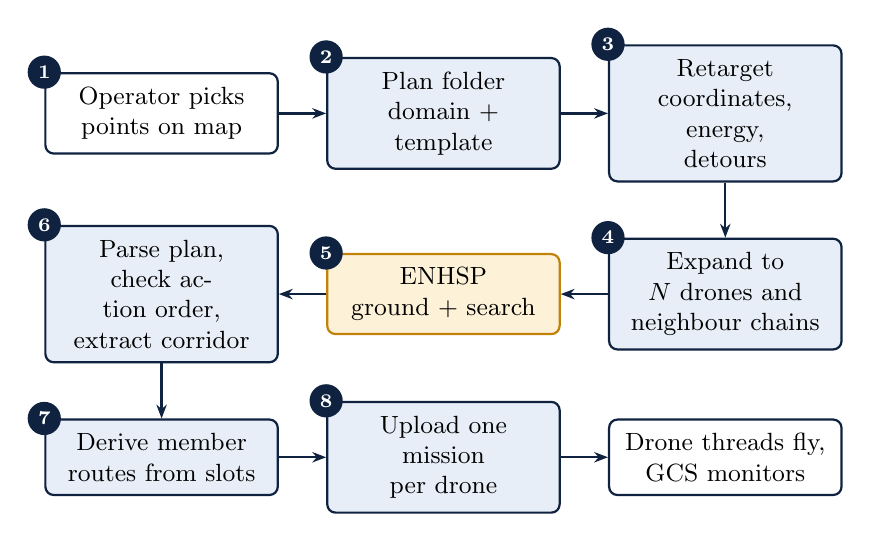
\begin{tikzpicture}[node distance=7mm and 6mm,
    stepnum/.style={circle,fill=navy,text=white,font=\scriptsize\bfseries,inner sep=1.2pt,minimum size=12pt}]
  \node[gbox,text width=2.6cm] (gui) {Operator picks\\points on map};
  \node[box,right=of gui,text width=2.6cm] (tpl) {Plan folder\\domain + template};
  \node[box,right=of tpl,text width=2.6cm] (ret) {Retarget\\coordinates, energy,\\detours};
  \node[box,below=of ret,text width=2.6cm] (exp) {Expand to\\$N$ drones and\\neighbour chains};
  \node[abox,left=of exp,text width=2.6cm] (enhsp) {ENHSP\\ground + search};
  \node[box,left=of enhsp,text width=2.6cm] (chk) {Parse plan,\\check action order,\\extract corridor};
  \node[box,below=of chk,text width=2.6cm] (der) {Derive member\\routes from slots};
  \node[box,right=of der,text width=2.6cm] (up) {Upload one mission\\per drone};
  \node[gbox,right=of up,text width=2.6cm] (fly) {Drone threads fly,\\GCS monitors};
  \draw[arr] (gui)--(tpl);
  \draw[arr] (tpl)--(ret);
  \draw[arr] (ret)--(exp);
  \draw[arr] (exp)--(enhsp);
  \draw[arr] (enhsp)--(chk);
  \draw[arr] (chk)--(der);
  \draw[arr] (der)--(up);
  \draw[arr] (up)--(fly);
  \foreach \n/\s in {gui/1,tpl/2,ret/3,exp/4,enhsp/5,chk/6,der/7,up/8}
    \node[stepnum] at (\n.north west) {\s};
\end{tikzpicture}
\caption[The planning pipeline from map input to flight]{The planning pipeline, from the
operator's map input to the drones' flight. The numbers are the steps described above.}
\label{fig:pipeline}
\end{figure}

\section{Plan Kinds and Folders}
The plan service decides how to treat a plan from the \emph{domain name} written inside
\code{domain.pddl}, not from the folder name. This lets a folder be renamed freely and makes the
domain file the single source of truth. Table~\ref{tab:inventory} lists the fourteen simulator plans.

\begin{table}[H]
\caption{Inventory of the fourteen simulator mission plans}\label{tab:inventory}
\small
\begin{tabularx}{\textwidth}{@{}P{0.22\textwidth}>{\ttfamily\scriptsize}P{0.34\textwidth}P{0.23\textwidth}Y@{}}
\toprule
\textbf{Folder} & \textbf{\normalfont\small Domain name} & \textbf{Kind} & \textbf{Drones} \\
\midrule
\code{travell}           & swarm-drone-mission               & point\_to\_point    & 1 to \maxTravel \\
\code{Search}            & forest-drone-search               & area\_coverage      & 2 to \maxSearch \\
\code{vformation}        & v-formation-drone-mission         & formation           & odd, 3 to \maxV \\
\code{gridformation}     & grid-formation-drone-mission      & grid\_formation     & 4 to \maxGrid \\
\code{3dgridformation}   & cube-grid-formation-drone-mission & cube\_formation     & 8 to \maxCube \\
\code{parabolaformation} & parabola-formation-drone-mission  & parabola\_formation & exactly 3 \\
\code{figure8formation}  & figure8-formation-drone-mission   & figure8\_formation  & 2 to capacity \\
\code{starformation}     & star-formation-drone-mission      & star\_formation     & 6 to \maxStar \\
\code{planets}           & planets-formation-drone-mission   & planets\_formation  & 2 to \maxPlanets \\
\code{Inspect}           & road-inspection-drone-mission     & road\_inspection    & 1 \\
\code{BatteryAware} & battery-aware-drone-mission & battery\_aware & 1 \\
\code{Formula-4} & formula4-drone-mission & formula4\_formation & 4 \\
\code{Formation-Circle} & circle-formation-drone-mission & circle\_formation & 4 \\
\code{Task-Allocation} & task-allocation & task\_allocation & 4 \\
\bottomrule
\end{tabularx}
\end{table}

The folder \code{Task-Allocation} uses domain \code{task-allocation} and kind
\code{task\_allocation}. It needs exactly four selected drones and uses the drone-thread backend.
Its current code is described in Section~\ref{sec:plan-task}; its older README does not yet
describe this simulator support.

\section{Run Records}
Every planning request writes a time-stamped folder under \code{plans/<name>/runs/} containing
the exact problem that was solved and the full ENHSP output. These records made it possible to
trace every unsolvable request back to its input, and they are the source of the statistics in
Chapter~\ref{ch:results}.

%% =====================================================================
%%  CHAPTER 4  PDDL MODELLING APPROACH
%% =====================================================================
\chapter{PDDL Modelling Approach}\label{ch:model}

\section{A Shared Vocabulary}
A PDDL domain describes the world with two kinds of building blocks:
\begin{itemize}
  \item a \textbf{predicate} is a yes/no statement, like a light switch that is either on or off.
        For example, \code{(gps-ok drone1)} is either true or false;
  \item a \textbf{function} (numeric fluent) is a number that can go up and down, like a fuel
        gauge. For example, \code{(battery drone1)} may be 85.
\end{itemize}
Actions read these switches and gauges in their preconditions and change them in their effects.
To make the original plans easy to read together, I used the same names for the same idea in every
domain. A reader who understands one plan can therefore read any other. The domains declare the
types \code{drone}, \code{location} and \code{controller} (plus plan-specific types such as
\code{forest-area} or \code{layer}). Table~\ref{tab:vocab} lists the shared names and says in
simple words what each one means; \code{?d} stands for a drone and \code{?l}, \code{?a},
\code{?b} for places.

\begin{longtable}{@{}>{\ttfamily\footnotesize}P{0.36\textwidth}P{0.58\textwidth}@{}}
\caption{Shared predicates and numeric functions used across the domains}\label{tab:vocab}\\
\toprule
\normalfont\small\textbf{Name} & \textbf{Meaning in simple words} \\
\midrule
\endfirsthead
\toprule
\normalfont\small\textbf{Name} & \textbf{Meaning in simple words} \\
\midrule
\endhead
\bottomrule
\endfoot
\multicolumn{2}{@{}l}{\textit{\small Where a drone is and what it is doing (yes/no)}} \\
(at ?d ?l)              & The drone is at place \code{?l}. \\
(formation-at ?l)       & The whole formation is at place \code{?l}. \\
(landed ?d)             & The drone is on the ground. \\
(airborne ?d)           & The drone has taken off. \\
(flying ?d)             & The drone is moving on its mission. \\
(at-cruise-altitude ?d) & The drone has climbed to its own working height. \\
(connected ?a ?b)       & There is a straight leg from place \code{?a} to place \code{?b}. \\
(safe-route ?a ?b)      & That leg does not cross a no-fly area. \\
\midrule
\multicolumn{2}{@{}l}{\textit{\small Health and communication (yes/no)}} \\
(gps-ok ?d)             & The drone knows where it is: its GPS works. \\
(communication-ok ?d)   & The drone can talk to the ground station. \\
(neighbor-comm-ok ?d)   & The drone can talk to all its neighbours in the formation. \\
(drone-healthy ?d)      & The drone has passed its health check. \\
(gps-lost ?d)           & A GPS failure has been detected on this drone. \\
(communication-lost ?d) & A link failure has been detected on this drone. \\
(health-failure ?d)     & A health failure has been detected on this drone. \\
(controller-notified ?d)& The ground station has been told about the failure. \\
\midrule
\multicolumn{2}{@{}l}{\textit{\small Numbers that go up and down}} \\
(battery ?d)            & Charge left, on a scale where 100 means full. \\
(max-battery ?d)        & The charge of a full battery. \\
(minimum-return-battery ?d) & Charge that must always be kept to get home safely. \\
(distance ?a ?b)        & Length of a leg, in metres. \\
(energy-required ?a ?b) & Charge used to fly that leg. \\
(climb-energy ?d)       & Charge used to climb to working height. \\
(cruise-leg-energy ?d)  & Charge a follower uses for one leg of the formation. \\
(health ?d)             & Health score of the drone (full health is 100). \\
(minimum-health ?d)     & Lowest health score allowed for flying. \\
(altitude ?d)           & Current height of the drone. \\
(hover-altitude ?d)     & Height right after take-off. \\
(target-altitude ?d)    & Working (cruise) height of this drone. \\
(slot-along-offset ?d)  & How far behind the leader the drone flies, in metres. \\
(slot-cross-offset ?d)  & How far to the left or right of the leader it flies. \\
\end{longtable}

\section{The Common Mission Life Cycle}
Every formation plan follows the same life cycle (Figure~\ref{fig:lifecycle}). A drone first
passes a \code{pre-flight-check}, which needs it to be landed at the source with GPS, radio and
health in order and a battery above its return reserve. It then takes off to hover altitude and
climbs to its own cruise altitude, paying \code{climb-energy}. Once airborne, it takes its slot
in the formation. The establish action (for example \code{establish-v-formation}) fires only
when every member is in
its slot, at altitude and in contact with its neighbours. The leader then flies the corridor one
leg at a time with \code{formation-cruise}; after each leg the formation is marked ``open'' and
a close-up action (\code{close-up-wings}, \code{close-up-grid}, \code{hold-parabola-shape},
\code{follow-leader}) must bring every member back into its slot before the next leg. The
mission completes when the closed formation is at the destination.

\begin{figure}[H]
\centering
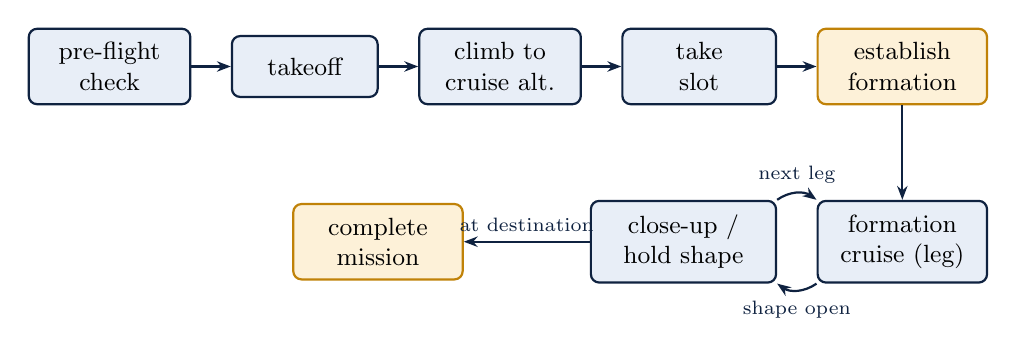
\begin{tikzpicture}[node distance=5mm and 5mm, every node/.style={font=\footnotesize}]
  \node[box,text width=1.7cm] (pf) {pre-flight\\check};
  \node[box,right=of pf,text width=1.5cm] (to) {takeoff};
  \node[box,right=of to,text width=1.7cm] (cl) {climb to\\cruise alt.};
  \node[box,right=of cl,text width=1.6cm] (sl) {take\\slot};
  \node[abox,right=of sl,text width=1.8cm] (es) {establish\\formation};
  \node[box,below=12mm of es,text width=1.8cm] (cr) {formation\\cruise (leg)};
  \node[box,left=of cr,text width=2.0cm] (cu) {close-up /\\hold shape};
  \node[abox,left=16mm of cu,text width=1.8cm] (cm) {complete\\mission};
  \draw[arr] (pf)--(to); \draw[arr] (to)--(cl); \draw[arr] (cl)--(sl); \draw[arr] (sl)--(es);
  \draw[arr] (es)--(cr);
  \draw[arr] (cr.south west) to[bend left=35] node[below,font=\scriptsize]{shape open} (cu.south east);
  \draw[arr] (cu.north east) to[bend left=35] node[above,font=\scriptsize]{next leg} (cr.north west);
  \draw[arr] (cu)--node[above,font=\scriptsize]{at destination}(cm);
\end{tikzpicture}
\caption[The life cycle shared by the formation plans]{The life cycle shared by the formation
plans. Each box is one PDDL action (or one action per drone).}
\label{fig:lifecycle}
\end{figure}

The take-off step itself is short but illustrates the style used throughout:

\begin{lstlisting}
(:action takeoff
    :parameters (?d - drone ?l - location)
    :precondition (and (at ?d ?l) (source ?l) (landed ?d)
                       (preflight-done ?d)
                       (gps-ok ?d) (communication-ok ?d) (drone-healthy ?d))
    :effect (and (not (landed ?d)) (airborne ?d) (flying ?d)
                 (assign (altitude ?d) (hover-altitude ?d))))
\end{lstlisting}

\noindent In words: a drone may take off only if it is on the ground at the source, has passed
its pre-flight check, and its GPS, radio and health are all fine. After take-off it is no longer
landed, it is airborne and flying, and its height is set to the hover height.

\section{Design Patterns for Tractable Swarm Models}
Swarm problems grow quickly with the number of drones: every extra drone adds more actions for
the planner to try. Four simple ideas kept the models small enough for ENHSP to solve within
seconds. Each is explained below as the problem, the idea, and why it helps.

\paragraph{1. Plan the leader, let the others follow}
\emph{The problem:} if the planner had to choose a route for every drone separately, its work
would grow very fast with each extra drone. \emph{The idea:} think of a mother duck and her
ducklings. Only the mother decides where to go; each duckling simply keeps its place behind her.
In the same way ENHSP plans only the leader's path. After every leg, one single action moves all
followers back into their places at once. The followers' real map routes are worked out
afterwards, outside the planner, by shifting the leader's route back and sideways by each
drone's slot. \emph{Why it helps:} the planning work grows only a little with each extra drone.

\paragraph{2. One ``can talk to my neighbours'' flag per drone}
\emph{The problem:} checking every \emph{pair} of drones is a lot of checks. A cube of 64 drones
has hundreds of neighbour pairs, and checking them all in every action would slow the planner
down. \emph{The idea:} the problem file still lists who is a neighbour of whom
(\code{wing-neighbor}, \code{grid-neighbor}, \code{cube-neighbor}, \code{train-neighbor},
\code{orbit-neighbor}), so that a person or the run time can read it. But the actions check only
one yes/no flag per drone, \code{neighbor-comm-ok}, which means ``this drone can talk to all of
its neighbours''. \emph{Why it helps:} the number of checks grows with the number of drones, not
with the number of pairs.

\paragraph{3. On/off steps instead of comparing two counters}
\emph{The problem:} the cube takes off layer by layer, bottom first. My first version used a
counter ``layers cleared so far'' and let a drone take off only when its own layer number was not
larger than that counter. ENHSP is poor at judging progress when two changing numbers are
compared with each other, so it searched almost blindly and a 25-drone cube did not finish in
90\,s. \emph{The idea:} think of a traffic light for each floor of a building. Each layer became
an object with a ``launched'' light, and a layer's light turns green only when the layer below
has fully climbed. \emph{Why it helps:} the planner can now see clear progress, and the same
problem was solved in about one second.

\paragraph{4. Write one fact per line in templates}
\emph{The problem:} the program that grows a template to $N$ drones copies it line by line. If
one fact is split over three lines, only part of it is copied and the new drone gets a broken
fact. \emph{The idea:} always write each per-drone fact on a single line, for example
\code{(= (hover-altitude drone-member) 2)}. \emph{Why it helps:} copying a line always copies a
whole fact. Breaking this rule caused the grid formation defect described in
Section~\ref{sec:defects}.

%% =====================================================================
%%  CHAPTER 5  MISSION PLANS
%% =====================================================================
\chapter{The Mission Plans}\label{ch:plans}
This chapter explains the plans using the following points:
\begin{itemize}
  \item \textbf{What the mission does}, in plain words, and an \emph{at a glance} box with its
        map input, number of drones and neighbours;
  \item \textbf{Communication}: a diagram of which drones talk to which, followed by the PDDL that
        expresses it;
  \item \textbf{Important PDDL}: only the actions that make this plan different from the others.
        The parts every plan shares (pre-flight check, take-off, climb, fault detection) are
        explained once, in Chapter~\ref{ch:model} and Chapter~\ref{ch:faults};
  \item \textbf{Action order}: the order in which ENHSP applies the actions;
  \item \textbf{Output}: what the plan looks like in the simulator.
\end{itemize}
Figure~\ref{fig:legend} explains the symbols used in all communication diagrams of this chapter.

\begin{figure}[H]
\centering
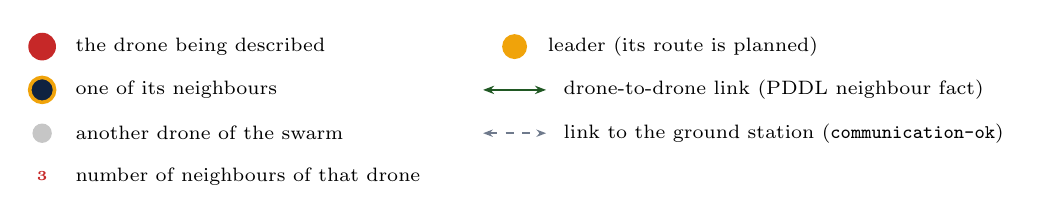
\begin{tikzpicture}[every node/.style={font=\scriptsize}]
  \node[focus] at (0,0) {};        \node[anchor=west] at (0.3,0) {the drone being described};
  \node[nbr] at (0,-0.55) {};      \node[anchor=west] at (0.3,-0.55) {one of its neighbours};
  \node[other] at (0,-1.1) {};     \node[anchor=west] at (0.3,-1.1) {another drone of the swarm};
  \node[leader] at (6.0,0) {};     \node[anchor=west] at (6.3,0) {leader (its route is planned)};
  \draw[comm] (5.6,-0.55)--(6.4,-0.55); \node[anchor=west] at (6.5,-0.55) {drone-to-drone link (PDDL neighbour fact)};
  \draw[glink] (5.6,-1.1)--(6.4,-1.1);  \node[anchor=west] at (6.5,-1.1) {link to the ground station (\code{communication-ok})};
  \node[cnt] at (0,-1.65) {3};     \node[anchor=west] at (0.3,-1.65) {number of neighbours of that drone};
\end{tikzpicture}
\caption[Symbols used in the communication diagrams]{Symbols used in the communication diagrams.
Every drone in the simulator plans also has a ground-station link, even where it is not drawn.}
\label{fig:legend}
\end{figure}

%% ---------------------------------------------------------------------
\section{Point-to-Point Travel}\label{sec:plan-travel}
\paragraph{What the mission does}
The whole selected swarm flies one shared route from a picked source to a picked destination.
If the operator marks a no-fly area across the direct line, the route goes around it through
detour waypoints. The template has a single drone, \code{drone1}, which is copied once for every
selected drone, so every drone gets its own checks and its own legs in the plan. This is the base
domain of the project, and it also contains the most complete fault handling
(Chapter~\ref{ch:faults}).

\glancebox{At a glance: point-to-point travel}{
Map input & source, destination, optional no-fly area \\
Drones & 1 to \maxTravel{}, any number in between \\
Neighbours per drone & none -- each drone talks only to the ground station \\
ENHSP plans & every drone's legs \\
Special feature & battery check before every leg; full ground-controller fault responses \\}

\paragraph{Communication}
The drones fly the same route independently and do not depend on each other, so no
drone-to-drone links are needed. Each drone has exactly one link, to the ground station
(Figure~\ref{fig:comm-travel}).

\begin{figure}[H]
\centering
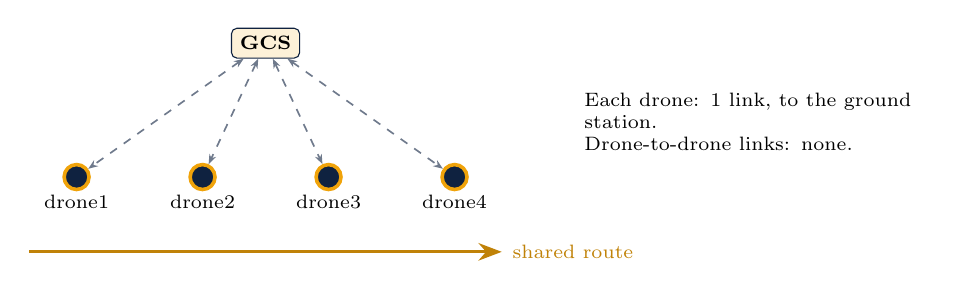
\begin{tikzpicture}
  \node[gcs] (g) at (0,1.7) {GCS};
  \foreach \i/\x in {1/-2.4,2/-0.8,3/0.8,4/2.4} {
    \node[nbr] (d\i) at (\x,0) {};
    \node[font=\scriptsize,below=3pt] at (d\i) {drone\i};
    \draw[glink] (g)--(d\i);
  }
  \draw[amber!80!black,line width=1.2pt,-{Stealth}] (-3,-0.95)--(3,-0.95) node[right,font=\scriptsize]{shared route};
  \node[note] at (6.2,0.7) {Each drone: 1 link, to the ground station.\\Drone-to-drone links: none.};
\end{tikzpicture}
\caption[Communication in point-to-point travel]{Communication in point-to-point travel: every
drone talks only to the ground station.}
\label{fig:comm-travel}
\end{figure}

\noindent In PDDL the ground link is the flag \code{communication-ok}. The problem starts with it
set for every drone, and the moving actions refuse to move a drone without it:

\begin{lstlisting}
;; problem: the template drone (copied for every drone) starts with a working link
(gps-ok drone1)
(communication-ok drone1)

;; domain: a leg is flown only while the link (and GPS, health, battery) is fine
(:action travel
    :parameters (?d - drone ?from - location ?to - location)
    :precondition (and (at ?d ?from) (route-planned ?d) (safe-route ?from ?to)
                       (gps-ok ?d) (communication-ok ?d) (drone-healthy ?d)
                       (> (battery ?d) (energy-required ?from ?to)))
    :effect (and (at ?d ?to) (not (at ?d ?from)) (flying ?d)
                 (decrease (battery ?d) (energy-required ?from ?to))
                 (not (route-planned ?d))))
\end{lstlisting}

\paragraph{Important PDDL}
Before each move a drone performs \code{check-distance} and \code{check-battery}; if the battery
cannot cover the leg, \code{notify-insufficient-battery} records the fact instead. A route is
planned only when every safety check passes:

\begin{lstlisting}
(:action plan-safe-route
    :parameters (?d - drone ?from - location ?to - location)
    :precondition (and (at ?d ?from) (connected ?from ?to) (safe-route ?from ?to)
                       (battery-checked ?d)
                       (gps-ok ?d) (communication-ok ?d) (drone-healthy ?d))
    :effect (route-planned ?d))
\end{lstlisting}

\noindent The \code{travel} action above clears \code{route-planned}, so the checks must be
repeated for every leg. A direct leg that crosses the no-fly area is marked
\code{restricted-route} and has no \code{safe-route} fact, so the planner has to use the detour
waypoints.

\needspace{6\baselineskip}
\paragraph{Action order}
For each drone:
\actionflow{check-distance \then check-battery \then plan-safe-route \then travel \then
reach-destination}
With detours, the middle three actions repeat once per leg.

\paragraph{Reading the ENHSP output}
Below is the complete output of one logged request with three drones and no no-fly area (the
lines in the middle of the search are shortened).

\recordlabel{ENHSP output --- point-to-point travel, three drones}
\begin{lstlisting}[style=plain]
Domain parsed
Problem parsed
Grounding..
Grounding Time: 26
|F|:24
|X|:3
|A|:36
h(I):27.0
 g(n)= 1.0 h(n)=25.0
 g(n)= 2.0 h(n)=23.0
 ...
 g(n)= 14.0 h(n)=1.0
Problem Solved

Found Plan:
0.0: (check-distance drone3 source destination)
1.0: (check-distance drone2 source waypoint1)
2.0: (check-distance drone1 source waypoint1)
3.0: (check-battery drone1 source waypoint1)
4.0: (check-battery drone2 source waypoint1)
5.0: (check-battery drone3 source destination)
6.0: (plan-safe-route drone3 source destination)
7.0: (plan-safe-route drone2 source destination)
8.0: (plan-safe-route drone1 source destination)
9.0: (travel drone2 source destination)
10.0: (travel drone1 source destination)
11.0: (travel drone3 source destination)
12.0: (reach-destination drone2 destination)
13.0: (reach-destination drone1 destination)
14.0: (reach-destination drone3 destination)

Plan-Length:15
Planning Time (msec): 34
Expanded Nodes:16
States Evaluated:43
\end{lstlisting}

\noindent The output has three parts.

\begin{enumerate}[leftmargin=*]
  \item \textbf{Preparation.} ENHSP reads the two files and then \emph{grounds} them: it replaces
        every \code{?d}, \code{?from} and \code{?to} by real drones and places, producing every
        concrete action (26\,ms here). \code{|F|:24} means there are 24 yes/no facts,
        \code{|X|:3} means there are 3 numbers (the battery of each drone) and \code{|A|:36}
        means there are 36 concrete actions to choose from.
  \item \textbf{Search.} \code{h(I):27.0} is ENHSP's estimate of how far the start is from the
        goal. Each line \code{g(n)= \ldots{} h(n)= \ldots} shows the number of actions chosen so
        far ($g$) and the estimated number still needed ($h$). Here $h$ falls steadily from 25
        to 1, which means the search went straight to the goal without getting lost.
  \item \textbf{The plan.} Each line has the form \code{step: (action arguments)}. The number
        before the colon is the \emph{position} of the action in the plan (0, 1, 2, \ldots), not
        a time in seconds. Reading only the lines of \code{drone1} gives its own story: it checks
        the distance, checks its battery, plans a safe route, travels from the source to the
        destination and reaches the destination. ENHSP mixes the three drones together because
        their order does not matter; the plan service separates them again by drone.
        \code{Plan-Length:15} is five actions for each of the three drones, found in 34\,ms after
        evaluating only 43 states.
\end{enumerate}

\noindent One detail is worth noticing: \code{drone1} and \code{drone2} checked their battery
against the leg to \code{waypoint1} but then flew straight to the destination. This is allowed
because the check flags belong to the drone, not to one leg. It is still safe, because the
\code{travel} action itself checks again that the battery covers the leg that is actually flown.

\screenshot{travel.png}{Point-to-point travel in the simulator}{Point-to-point travel in the
simulator: the shared route from source to destination, flown by all selected drones.}{fig:out-travel}

%% ---------------------------------------------------------------------
\section{Forest Area Search}\label{sec:plan-search}
\paragraph{What the mission does}
The operator clicks a base point and the corners of a forest area. The area is split into equal
lanes, one per drone, and each lane is covered by a back-and-forth (``lawnmower'') path. Every
drone takes off from the common base, flies to its own lane, covers it, and returns to the base.
Unlike travel, each drone has its own route. At least two drones are needed.

\glancebox{At a glance: forest area search}{
Map input & base point, corners of the forest area \\
Drones & 2 to \maxSearch{} (one lane per drone) \\
Neighbours per drone & none -- ground station link, plus a separation check against every
other drone \\
ENHSP plans & one lane per drone, out and back \\
Special feature & pairwise minimum separation of 10\,m; low-battery return \\}

\paragraph{Communication}
Each drone talks only to the ground station. The drones do not exchange messages, but the
planner makes sure that no two drones come closer than a minimum separation
(Figure~\ref{fig:comm-search}).

\begin{figure}[H]
\centering
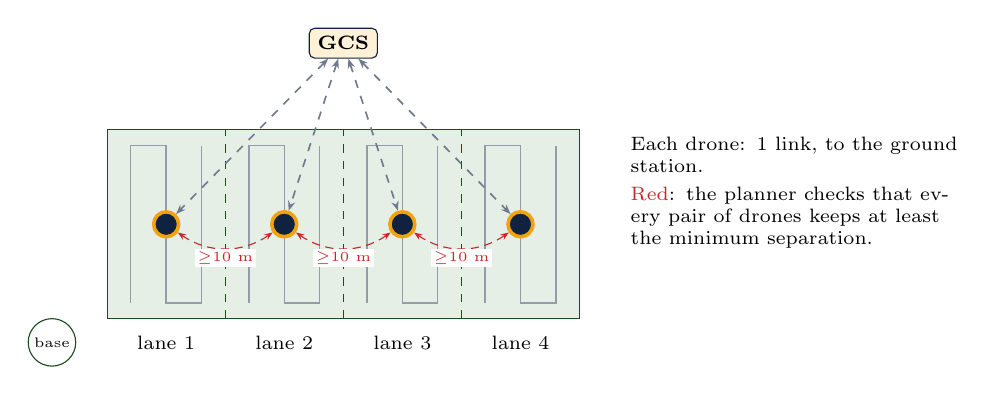
\begin{tikzpicture}
  \fill[okgreen!12] (0,0) rectangle (6,2.4);
  \draw[okgreen!60!black] (0,0) rectangle (6,2.4);
  \foreach \k in {1,2,3} \draw[okgreen!60!black,dashed] (1.5*\k,0)--(1.5*\k,2.4);
  \foreach \k in {0,1,2,3} {
    \draw[navy!45,line width=0.5pt] (1.5*\k+0.3,0.2)--(1.5*\k+0.3,2.2)--(1.5*\k+0.75,2.2)
      --(1.5*\k+0.75,0.2)--(1.5*\k+1.2,0.2)--(1.5*\k+1.2,2.2);
    \node[nbr] (s\k) at (1.5*\k+0.75,1.2) {};
    \pgfmathtruncatemacro{\lane}{\k+1}
    \node[font=\scriptsize] at (1.5*\k+0.75,-0.3) {lane \lane};
  }
  \foreach \a/\b in {0/1,1/2,2/3}
    \draw[warnred,{Stealth[length=3pt]}-{Stealth[length=3pt]},densely dashed] (s\a) to[bend right=35]
      node[below,font=\tiny,fill=white,inner sep=1pt]{$\geq$10 m} (s\b);
  \node[gcs] (g) at (3,3.5) {GCS};
  \foreach \k in {0,1,2,3} \draw[glink] (g)--(s\k);
  \node[circle,draw=okgreen!60!black,fill=white,font=\tiny,inner sep=1.5pt] at (-0.7,-0.3) {base};
  \node[note] at (8.8,1.6) {Each drone: 1 link, to the ground station.\\[2pt]
    {\color{warnred}Red}: the planner checks that every pair of drones keeps at least the
    minimum separation.};
\end{tikzpicture}
\caption[Communication in forest area search]{Communication in forest area search: ground links
only, plus a separation check between drones.}
\label{fig:comm-search}
\end{figure}

\noindent In PDDL the separation is a number for every pair of drones, and an action confirms
that the pair is far enough apart. The covering action needs the drone's ground link:

\begin{lstlisting}
;; problem: minimum distance between the two template drones, in metres
(= (minimum-drone-separation drone1 drone2) 10)
(= (minimum-drone-separation drone2 drone1) 10)

;; domain: a pair of drones is marked safe only if they are far enough apart
(:action check-drone-separation
    :parameters (?d1 - drone ?d2 - drone ?l1 - location ?l2 - location)
    :precondition (and (at ?d1 ?l1) (at ?d2 ?l2) (not (= ?d1 ?d2))
                       (>= (distance ?l1 ?l2) (minimum-drone-separation ?d1 ?d2)))
    :effect (and (safe-separation ?d1 ?d2) (separation-ok ?d1) (separation-ok ?d2)))
\end{lstlisting}

\paragraph{Important PDDL}
The type \code{forest-area} represents a lane, and \code{(assigned ?d ?a)} gives each drone its
own lane. A lane is marked covered only by the drone assigned to it, while its GPS, link and
health are fine:

\begin{lstlisting}
(:action cover-area
    :parameters (?d - drone ?a - forest-area ?l - location)
    :precondition (and (at ?d ?l) (forest ?a) (area-location ?a ?l) (assigned ?d ?a)
                       (searching ?d) (not (area-covered ?a))
                       (gps-ok ?d) (communication-ok ?d) (drone-healthy ?d))
    :effect (and (area-covered ?a) (search-completed ?d) (not (searching ?d))))
\end{lstlisting}

\noindent An \code{emergency-low-battery-return} action marks a drone as returning whenever its
battery falls to the return reserve.

\needspace{6\baselineskip}
\paragraph{Action order}
For each drone:
\actionflow{check-battery \then start-search \then move-search (repeated along the lane) \then
cover-area \then complete-forest-search \then return-to-base \then complete-drone-mission}

\screenshot{search.png}{Forest area search in the simulator}{Forest area search in the
simulator: the marked area split into one lane per drone.}{fig:out-search}

%% ---------------------------------------------------------------------
\section{V Formation}\label{sec:plan-v}
\paragraph{What the mission does}
The operator picks points as for travel. A leader (the apex) flies the corridor and the other
drones form two wings behind it, like a flock of birds. Each rank sits 17.32\,m back and 20\,m
to the side of the one before it, so the wing angle is $60^\circ$ (Figure~\ref{fig:vgrid}a).
The number of drones must be odd: one leader plus the same number on each wing. Extra drones add
further ranks. The leader takes off first and the wings follow after a short delay.

\glancebox{At a glance: V formation}{
Map input & source, destination, optional no-fly area \\
Drones & odd numbers, 3 to \maxV{} \\
Neighbours per drone & 1 or 2 -- the drone in front and the drone behind on its wing \\
ENHSP plans & the leader's corridor \\
Special feature & timed wing launch; wings close up after every leg \\}

\paragraph{Communication}
Each wing is a chain. A drone talks to the drone in front of it and the drone behind it on the
same wing. The leader talks to the first drone of each wing (Figure~\ref{fig:comm-v}).

\begin{figure}[H]
\centering
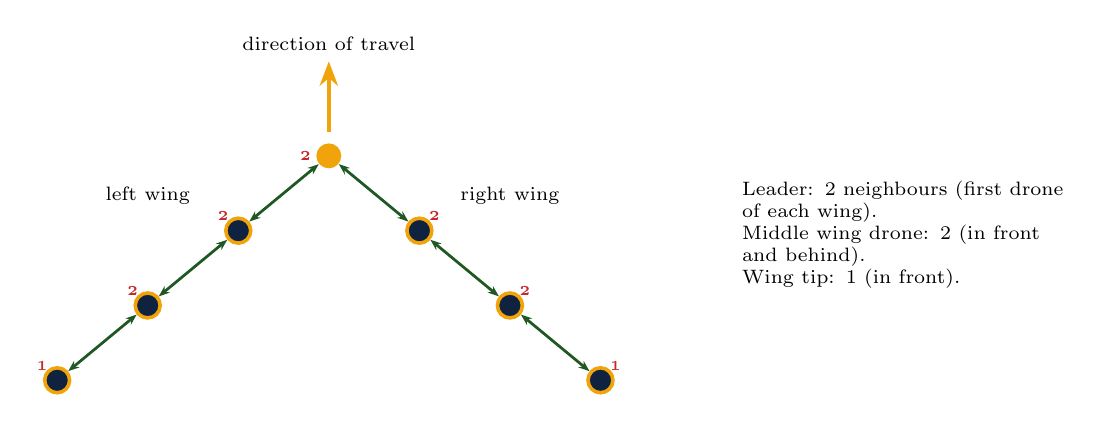
\begin{tikzpicture}
  \draw[amber,line width=1.3pt,-{Stealth}] (0,0.3)--(0,1.2) node[above,font=\scriptsize,black]{direction of travel};
  \node[leader] (L) at (0,0) {};
  \foreach \i in {1,2,3} {
    \node[nbr] (l\i) at (-\i*1.15,-\i*0.95) {};
    \node[nbr] (r\i) at (\i*1.15,-\i*0.95) {};
  }
  \draw[comm] (L)--(l1); \draw[comm] (l1)--(l2); \draw[comm] (l2)--(l3);
  \draw[comm] (L)--(r1); \draw[comm] (r1)--(r2); \draw[comm] (r2)--(r3);
  \node[cnt,left=3pt] at (L) {2};
  \foreach \i/\n in {1/2,2/2,3/1} {
    \node[cnt,above left=0pt] at (l\i) {\n};
    \node[cnt,above right=0pt] at (r\i) {\n};
  }
  \node[font=\scriptsize] at (-2.3,-0.5) {left wing};
  \node[font=\scriptsize] at (2.3,-0.5) {right wing};
  \node[note] at (7.4,-1.0) {Leader: 2 neighbours (first drone of each wing).\\
    Middle wing drone: 2 (in front and behind).\\Wing tip: 1 (in front).};
\end{tikzpicture}
\caption[Communication in the V formation]{Communication in the V formation: each wing is a
chain of neighbours starting at the leader.}
\label{fig:comm-v}
\end{figure}

\noindent In PDDL the chain is written as \code{wing-neighbor} facts in both directions, and
every drone has the \code{neighbor-comm-ok} flag. The formation can only be established when
every wing drone has that flag:

\begin{lstlisting}
;; problem: leader <-> rank 1 on each side (the expansion code adds rank 1 <-> rank 2, ...)
(wing-neighbor drone-lead drone-left)
(wing-neighbor drone-left drone-lead)
(wing-neighbor drone-lead drone-right)
(wing-neighbor drone-right drone-lead)
(neighbor-comm-ok drone-lead)
(neighbor-comm-ok drone-left)
(neighbor-comm-ok drone-right)

;; domain: the V is formed only if every wing drone is in place AND in contact
(:action establish-v-formation
    :parameters (?lead - drone ?l - location)
    :precondition (and (formation-leader ?lead) (slot-apex ?lead) (in-formation ?lead)
                       (at ?lead ?l) (at-cruise-altitude ?lead) (neighbor-comm-ok ?lead)
                       (forall (?w - drone)
                           (or (not (wing-drone ?w))
                               (and (in-formation ?w) (at ?w ?l)
                                    (at-cruise-altitude ?w) (neighbor-comm-ok ?w)))))
    :effect (and (v-formation-established) (formation-at ?l) (wings-closed)))
\end{lstlisting}

\paragraph{Important PDDL}
The timed launch uses a counter. While the airborne leader waits, \code{hold-position} adds one
second until the wing launch delay is reached; only then may the wing drones take off:

\begin{lstlisting}
(:action hold-position
    :parameters (?lead - drone)
    :precondition (and (formation-leader ?lead) (airborne ?lead)
                       (< (seconds-since-leader-airborne) (wing-launch-delay))
                       (gps-ok ?lead) (communication-ok ?lead) (drone-healthy ?lead))
    :effect (increase (seconds-since-leader-airborne) 1))
\end{lstlisting}

\noindent After each leg, \code{close-up-wings} moves every wing drone to the leader's new
location in one step, using a quantified conditional effect, and charges each of them
\code{cruise-leg-energy}.

\needspace{6\baselineskip}
\paragraph{Action order} ENHSP applies the actions in this order:
\actionflow{pre-flight-check, takeoff, climb (leader) \then hold-position (until the delay) \then
pre-flight-check, takeoff, climb (each wing drone) \then take-formation-slot (each drone) \then
establish-v-formation \then [formation-cruise \then close-up-wings] for every leg \then
complete-formation-mission}

\screenshot{vformation.png}{V formation in the simulator}{V formation in the simulator: the
leader's corridor and the wing routes derived from it.}{fig:out-v}

%% ---------------------------------------------------------------------
\section{Two-Dimensional Grid Formation}\label{sec:plan-grid}
\paragraph{What the mission does}
The drones fly as a flat grid, 10\,m apart in every direction (Figure~\ref{fig:vgrid}b). A square
number of drones gives a square grid; otherwise the most square rectangle that fits the number
exactly is used (for example 12 drones become $3\times4$). At least four drones are needed. The
leader flies in the front row and the rest of the grid moves with it.

\glancebox{At a glance: two-dimensional grid}{
Map input & source, destination, optional no-fly area \\
Drones & 4 to \maxGrid{} \\
Neighbours per drone & 2 to 4 -- front, back, left and right \\
ENHSP plans & the leader's corridor \\
Special feature & grid shape chosen from the drone count; close-up after every leg \\}

\paragraph{Communication}
Each drone talks only to the drones directly in front, behind, to the left and to the right.
A corner drone therefore has 2 neighbours, an edge drone 3 and an inner drone 4
(Figure~\ref{fig:comm-grid}).

\begin{figure}[H]
\centering
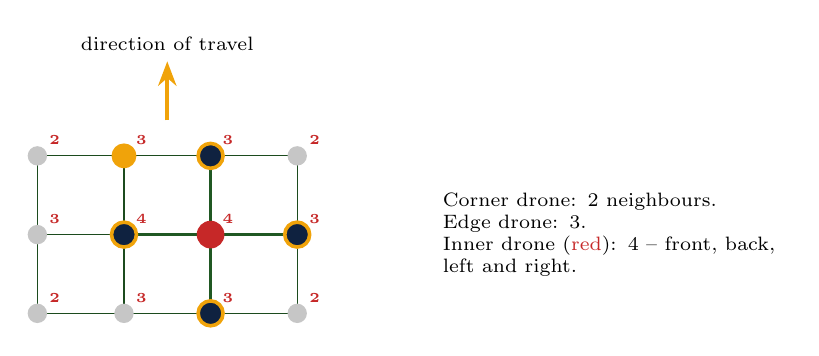
\begin{tikzpicture}
  \foreach \r in {0,1,2} \foreach \c in {0,...,3} \coordinate (q\r\c) at (\c*1.1,-\r*1.0);
  \foreach \r in {0,1,2} \draw[commthin] (q\r0)--(q\r3);
  \foreach \c in {0,...,3} \draw[commthin] (q0\c)--(q2\c);
  \draw[comm] (q12)--(q02); \draw[comm] (q12)--(q22); \draw[comm] (q12)--(q11); \draw[comm] (q12)--(q13);
  \foreach \r in {0,1,2} \foreach \c in {0,...,3} {
    \pgfmathtruncatemacro{\n}{(\r>0)+(\r<2)+(\c>0)+(\c<3)}
    \node[other] at (q\r\c) {};
    \node[cnt] at ($(q\r\c)+(0.22,0.2)$) {\n};
  }
  \foreach \p in {q02,q22,q11,q13} \node[nbr] at (\p) {};
  \node[leader] at (q01) {};
  \node[focus] at (q12) {};
  \draw[amber,line width=1.3pt,-{Stealth}] (1.65,0.45)--(1.65,1.2) node[above,font=\scriptsize,black]{direction of travel};
  \node[note] at (7.3,-1.0) {Corner drone: 2 neighbours.\\Edge drone: 3.\\Inner drone
    ({\color{warnred}red}): 4 -- front, back, left and right.};
\end{tikzpicture}
\caption[Communication in the grid formation]{Communication in the grid formation: each drone
talks to at most four drones next to it.}
\label{fig:comm-grid}
\end{figure}

\noindent In PDDL this is the \code{grid-neighbor} relation. The close-up after every leg checks
that every member still has its \code{neighbor-comm-ok} flag:

\begin{lstlisting}
;; problem: one neighbour pair of the template (rebuilt for the full grid on expansion)
(grid-neighbor drone-lead drone-member)
(grid-neighbor drone-member drone-lead)
(neighbor-comm-ok drone-lead)
(neighbor-comm-ok drone-member)

;; domain: after a leg, the grid is closed again only if every member is still fine
(:action close-up-grid
    :parameters (?lead - drone ?to - location)
    :precondition (and (grid-formation-established) (not (grid-closed))
                       (formation-leader ?lead) (formation-at ?to) (at ?lead ?to)
                       (forall (?m - drone)
                           (or (not (grid-member ?m))
                               (and (in-formation ?m) (at-cruise-altitude ?m)
                                    (gps-ok ?m) (communication-ok ?m) (drone-healthy ?m)
                                    (neighbor-comm-ok ?m)
                                    (> (battery ?m) (cruise-leg-energy ?m))))))
    :effect (and (forall (?m - drone) (when (grid-member ?m) (at ?m ?to)))
                 (forall (?m - drone)
                     (when (grid-member ?m) (decrease (battery ?m) (cruise-leg-energy ?m))))
                 (grid-closed)))
\end{lstlisting}

\paragraph{Important PDDL}
The grid differs from the V mainly in its slot offsets and neighbour relation: every member has
its own \code{slot-along-offset} and \code{slot-cross-offset} (multiples of 10\,m), and the
close-up action above is the only action that moves members. Because the planner moves all
members in one action, the plan length grows by only about four actions per extra drone.

\needspace{6\baselineskip}
\paragraph{Action order} ENHSP applies the actions in this order:
\actionflow{pre-flight-check, takeoff, climb (leader) \then hold-position \then pre-flight-check,
takeoff, climb (each member) \then take-grid-slot (each drone) \then establish-grid-formation
\then [formation-cruise \then close-up-grid] for every leg \then complete-grid-mission}

\begin{figure}[H]
\centering
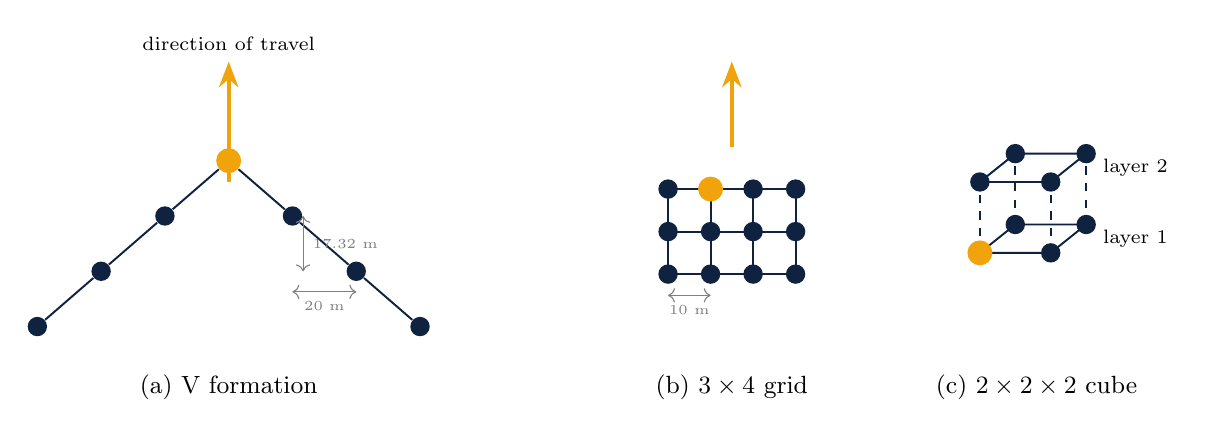
\begin{tikzpicture}[scale=0.9]
  % (a) V formation
  \begin{scope}
    \draw[amber,line width=1.4pt,-{Stealth}] (0,-0.3)--(0,1.4) node[above,font=\scriptsize,black]{direction of travel};
    \node[leader] (L) at (0,0) {};
    \foreach \i in {1,2,3} {
      \node[drone] (l\i) at (-\i*0.9,-\i*0.78) {};
      \node[drone] (r\i) at (\i*0.9,-\i*0.78) {};
    }
    \draw[link] (L)--(l1)--(l2)--(l3); \draw[link] (L)--(r1)--(r2)--(r3);
    \draw[<->,gray,thin] (1.05,-0.78)--(1.05,-1.56) node[midway,right,font=\tiny]{17.32 m};
    \draw[<->,gray,thin] (0.9,-1.85)--(1.8,-1.85) node[midway,below,font=\tiny]{20 m};
    \node[font=\small] at (0,-3.2) {(a) V formation};
  \end{scope}
  % (b) grid
  \begin{scope}[xshift=6.2cm,yshift=-0.4cm]
    \draw[amber,line width=1.4pt,-{Stealth}] (0.9,0.6)--(0.9,1.8);
    \foreach \r in {0,1,2} \foreach \c in {0,1,2,3} {
      \coordinate (g\r\c) at (\c*0.6,-\r*0.6);
    }
    \foreach \r in {0,1,2} { \draw[link] (g\r0)--(g\r3); }
    \foreach \c in {0,1,2,3} { \draw[link] (g0\c)--(g2\c); }
    \foreach \r in {0,1,2} \foreach \c in {0,1,2,3} { \node[drone] at (g\r\c) {}; }
    \node[leader] at (g01) {};
    \draw[<->,gray,thin] (0,-1.5)--(0.6,-1.5) node[midway,below,font=\tiny]{10 m};
    \node[font=\small] at (0.9,-2.8) {(b) $3\times4$ grid};
  \end{scope}
  % (c) cube
  \begin{scope}[xshift=10.6cm,yshift=-1.3cm]
    \foreach \z in {0,1} \foreach \x in {0,1} \foreach \y in {0,1}
      \coordinate (c\x\y\z) at ({\x*1.0+\y*0.5},{\z*1.0+\y*0.4});
    \foreach \z in {0,1} {
      \draw[link] (c00\z)--(c10\z)--(c11\z)--(c01\z)--cycle; }
    \foreach \x in {0,1} \foreach \y in {0,1} { \draw[link,dashed] (c\x\y0)--(c\x\y1); }
    \foreach \z in {0,1} \foreach \x in {0,1} \foreach \y in {0,1} { \node[drone] at (c\x\y\z) {}; }
    \node[leader] at (c000) {};
    \node[font=\scriptsize,right] at (1.6,0.2) {layer 1};
    \node[font=\scriptsize,right] at (1.6,1.2) {layer 2};
    \node[font=\small] at (0.8,-1.9) {(c) $2\times2\times2$ cube};
  \end{scope}
\end{tikzpicture}
\caption[Rigid formations: V, grid and cube]{Rigid formations. The amber drone is the leader
whose corridor ENHSP plans; lines show the neighbour links each drone must keep. In the cube,
vertical layers are separated by height.}
\label{fig:vgrid}
\end{figure}

\screenshot{grid.png}{Grid formation in the simulator}{Grid formation in the simulator: one route
per grid cell, parallel to the leader's corridor.}{fig:out-grid}

%% ---------------------------------------------------------------------
\section{Three-Dimensional Cube Formation}\label{sec:plan-cube}
\paragraph{What the mission does}
The grid extended upwards: a solid block of drones flies one corridor, 10\,m apart horizontally
and vertically (Figure~\ref{fig:vgrid}c). A square footprint is chosen and as many layers as
needed are stacked, allowing a partly filled top layer (for example 9 drones become
$3\times2\times2$ with 9 of 12 cells filled; 25 become $3\times3\times3$). At least eight drones
are needed. To avoid collisions while climbing, the block takes off layer by layer: the bottom
layer first, and each next layer only when the one below has reached its height.

\glancebox{At a glance: cube formation}{
Map input & source, destination, optional no-fly area \\
Drones & 8 to \maxCube{} \\
Neighbours per drone & up to 24 -- the surrounding $3\times3\times3$ block, except directly
above and below \\
ENHSP plans & the leader's corridor and the layer-by-layer launch \\
Special feature & each layer at its own height; layer gates for the climb \\}

\paragraph{Communication}
A drone talks to the drones around it in its own layer (up to 8) and in the layers just above
and below (up to 8 each). The drones directly above and below are not counted as neighbours,
because the vertical spacing alone keeps them apart. That gives up to 24 neighbours
(Figure~\ref{fig:comm-cube}).

\begin{figure}[H]
\centering
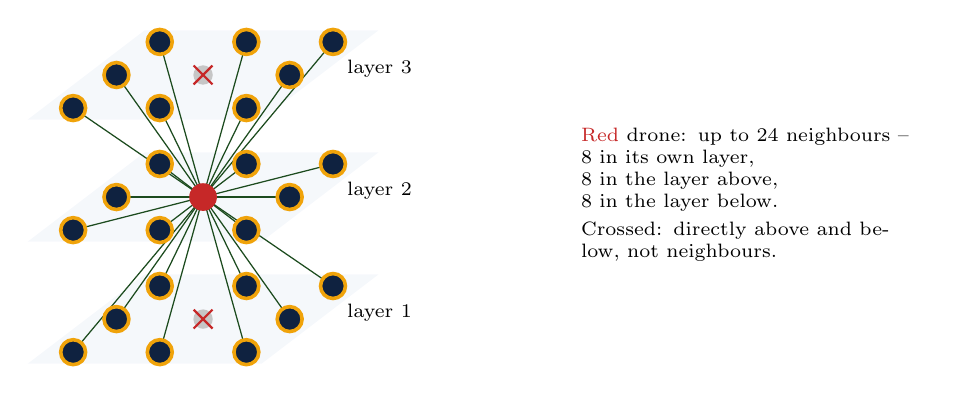
\begin{tikzpicture}
  \def\P(#1,#2,#3){({#2*1.1+#1*0.55},{#3*1.55+#1*0.42})}
  \coordinate (F) at ({1*1.1+1*0.55},{1*1.55+1*0.42});
  \foreach \z in {0,1,2} {
    \fill[softblue!70,opacity=0.6] ({-0.35*1.1-0.35*0.55},{\z*1.55-0.35*0.42})
      --({2.35*1.1-0.35*0.55},{\z*1.55-0.35*0.42})
      --({2.35*1.1+2.35*0.55},{\z*1.55+2.35*0.42})
      --({-0.35*1.1+2.35*0.55},{\z*1.55+2.35*0.42})--cycle;
    \pgfmathtruncatemacro{\lay}{\z+1}
    \node[font=\scriptsize,anchor=west] at ({2.45*1.1+1.2*0.55},{\z*1.55+0.5}) {layer \lay};
  }
  \foreach \z in {0,1,2} \foreach \r in {0,1,2} \foreach \c in {0,1,2} {
    \pgfmathtruncatemacro{\mid}{and(\r==1,\c==1)}
    \ifnum\mid=0 \draw[commthin] (F)--({\c*1.1+\r*0.55},{\z*1.55+\r*0.42}); \fi
  }
  \foreach \z in {0,1,2} \foreach \r in {2,1,0} \foreach \c in {0,1,2} {
    \pgfmathtruncatemacro{\mid}{and(\r==1,\c==1)}
    \ifnum\mid=1
      \ifnum\z=1 \node[focus] at ({\c*1.1+\r*0.55},{\z*1.55+\r*0.42}) {};
      \else
        \node[other] (x\z) at ({\c*1.1+\r*0.55},{\z*1.55+\r*0.42}) {};
        \draw[warnred,line width=0.8pt] ($(x\z)+(-0.12,-0.12)$)--($(x\z)+(0.12,0.12)$);
        \draw[warnred,line width=0.8pt] ($(x\z)+(-0.12,0.12)$)--($(x\z)+(0.12,-0.12)$);
      \fi
    \else
      \node[nbr] at ({\c*1.1+\r*0.55},{\z*1.55+\r*0.42}) {};
    \fi
  }
  \node[note] at (8.6,2.0) {{\color{warnred}Red} drone: up to 24 neighbours --\\
    8 in its own layer,\\8 in the layer above,\\8 in the layer below.\\[2pt]
    Crossed: directly above and below, not neighbours.};
\end{tikzpicture}
\caption[Communication in the cube formation]{Communication in the cube formation: up to 24
neighbours in the surrounding block.}
\label{fig:comm-cube}
\end{figure}

\noindent In PDDL the neighbours are \code{cube-neighbor} facts, and, as in the grid, the
formation is established only when every member has \code{neighbor-comm-ok}. The cube adds one
more condition: every layer must already have been launched:

\begin{lstlisting}
;; problem: one neighbour pair of the template (all 24-neighbour pairs added on expansion)
(cube-neighbor drone-lead drone-member)
(cube-neighbor drone-member drone-lead)
(neighbor-comm-ok drone-lead)
(neighbor-comm-ok drone-member)

;; domain: the block is formed only when all layers are up and every member is in contact
(:action establish-cube-formation
    :parameters (?lead - drone ?l - location)
    :precondition (and (formation-leader ?lead) (in-formation ?lead) (at ?lead ?l)
                       (at-cruise-altitude ?lead) (neighbor-comm-ok ?lead)
                       (forall (?ly - layer) (layer-launched ?ly))
                       (forall (?m - drone)
                           (or (not (cube-member ?m))
                               (and (in-formation ?m) (at ?m ?l)
                                    (at-cruise-altitude ?m) (neighbor-comm-ok ?m)))))
    :effect (and (cube-formation-established) (formation-at ?l) (cube-closed)))
\end{lstlisting}

\paragraph{Important PDDL}
Layers are separated by height, so each drone has its own \code{target-altitude} (base plus
10\,m per layer), and the run-time route adds a per-drone altitude offset. The swarm climbs
layer by layer using the ``traffic light'' pattern of Chapter~\ref{ch:model}. A layer is opened
only when every drone of the layer below has reached its height, and opening it clears all of
its drones for take-off:

\begin{lstlisting}
(:action open-next-layer
    :parameters (?lo - layer ?hi - layer)
    :precondition (and (layer-below ?lo ?hi) (layer-launched ?lo)
                       (not (layer-launched ?hi))
                       (forall (?d - drone)
                           (or (not (in-layer ?d ?lo)) (at-cruise-altitude ?d))))
    :effect (and (layer-launched ?hi)
                 (forall (?d - drone)
                     (when (in-layer ?d ?hi) (cleared-to-launch ?d)))))
\end{lstlisting}

\noindent Collision avoidance is built into the structure: fixed spacing, layer-by-layer ascent
and a \code{cube-closed} interlock that must hold before each leg.

\needspace{6\baselineskip}
\paragraph{Action order} ENHSP applies the actions in this order:
\actionflow{launch layer 1 (pre-flight-check, takeoff, climb for each drone) \then
open-next-layer \then launch layer 2 \then \ldots{} \then take-cube-slot (each drone) \then
establish-cube-formation \then [formation-cruise \then close-up-cube] for every leg \then
complete-cube-mission}

\screenshot{cube.png}{Cube formation in the simulator}{Cube formation in the simulator: the
layers of the block flying one corridor at different heights.}{fig:out-cube}

%% ---------------------------------------------------------------------
\section{Parabola Formation}\label{sec:plan-parabola}
\paragraph{What the mission does}
Three drones fly side by side on one line across the route, 10\,m apart. The middle drone (the
vertex) cruises at 50\,m and the two arm drones at 60\,m, so seen from behind they form an
upward-opening parabola (Figure~\ref{fig:parabola}). Extra selected drones stay on the ground.
This plan has the most detailed communication model: the drones must set up radio links with
each other, within range, before they may take their places.

\glancebox{At a glance: parabola formation}{
Map input & source, destination, optional no-fly area \\
Drones & exactly 3 \\
Neighbours per drone & 2 -- every drone talks to both others (6 directed links) \\
ENHSP plans & the vertex corridor and every link set-up \\
Special feature & range-checked links; the shape itself is checked in PDDL \\}

\paragraph{Communication}
All three pairs keep a direct link, in both directions, so there are six directed links
(Figure~\ref{fig:comm-parabola}). A link can only be set up when the two drones are within the
communication range of 100\,m.

\begin{figure}[H]
\centering
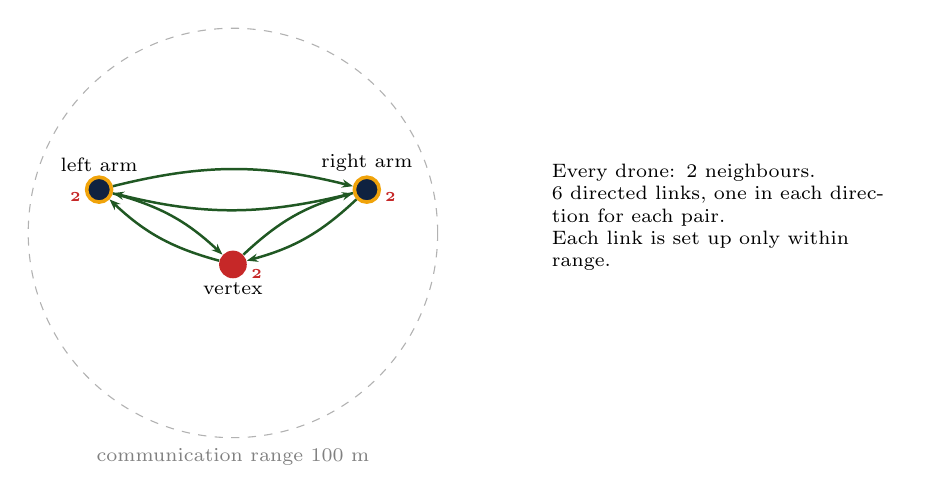
\begin{tikzpicture}
  \draw[gray!60,dashed] (0,0) circle (2.6);
  \node[font=\scriptsize,gray] at (0,-2.85) {communication range 100 m};
  \node[focus] (v) at (0,-0.4) {};
  \node[nbr] (a) at (-1.7,0.55) {};
  \node[nbr] (b) at (1.7,0.55) {};
  \foreach \s/\t in {v/a,a/v,v/b,b/v,a/b,b/a}
    \draw[-{Stealth[length=4pt]},okgreen!70!black,line width=0.9pt] (\s) to[bend left=14] (\t);
  \node[font=\scriptsize,below=3pt] at (v) {vertex};
  \node[font=\scriptsize,above=3pt] at (a) {left arm};
  \node[font=\scriptsize,above=3pt] at (b) {right arm};
  \node[cnt] at ($(v)+(0.3,-0.12)$) {2};
  \node[cnt] at ($(a)+(-0.3,-0.1)$) {2};
  \node[cnt] at ($(b)+(0.3,-0.1)$) {2};
  \node[note] at (6.2,0.2) {Every drone: 2 neighbours.\\6 directed links, one in each
    direction for each pair.\\Each link is set up only within range.};
\end{tikzpicture}
\caption[Communication in the parabola formation]{Communication in the parabola formation: a full
mesh of six directed, range-checked links.}
\label{fig:comm-parabola}
\end{figure}

\noindent In PDDL, every directed link is a \code{parabola-neighbor} fact, and a link becomes
\code{link-up} only through \code{establish-comm-link}. A drone is ready only when it has a link
to every one of its neighbours:

\begin{lstlisting}
;; problem: all six directed neighbour pairs
(parabola-neighbor drone-vertex drone-left)   (parabola-neighbor drone-left drone-vertex)
(parabola-neighbor drone-vertex drone-right)  (parabola-neighbor drone-right drone-vertex)
(parabola-neighbor drone-left drone-right)    (parabola-neighbor drone-right drone-left)

;; domain: a link is set up only between airborne drones that are within range
(:action establish-comm-link
    :parameters (?d1 - drone ?d2 - drone)
    :precondition (and (parabola-neighbor ?d1 ?d2) (not (link-up ?d1 ?d2))
                       (airborne ?d1) (airborne ?d2)
                       (at-cruise-altitude ?d1) (at-cruise-altitude ?d2)
                       (communication-ok ?d1) (communication-ok ?d2)
                       (neighbor-comm-ok ?d1) (neighbor-comm-ok ?d2)
                       (<= (link-distance ?d1 ?d2) (comm-range)))
    :effect (link-up ?d1 ?d2))

;; domain: a drone is ready when every one of its links is up
(:action confirm-swarm-comm
    :parameters (?d - drone)
    :precondition (and (airborne ?d) (not (swarm-comm-ready ?d))
                       (communication-ok ?d) (neighbor-comm-ok ?d)
                       (forall (?n - drone)
                           (or (not (parabola-neighbor ?d ?n)) (link-up ?d ?n))))
    :effect (swarm-comm-ready ?d))
\end{lstlisting}

\paragraph{Important PDDL}
The formation action checks the shape itself: each arm's target altitude minus the vertex's must
equal \code{arm-rise} (10\,m), so a flat line, an upside-down U or lopsided arms give no plan,
and every vertex--arm gap (14.14\,m) must be at least \code{min-separation} (10\,m).

\begin{lstlisting}
(:action establish-parabola-formation
  :parameters (?vtx - drone ?l - location)
  :precondition (and (formation-leader ?vtx) (slot-vertex ?vtx) (in-formation ?vtx)
     (at ?vtx ?l) (at-cruise-altitude ?vtx) (swarm-comm-ready ?vtx)
     (forall (?a - drone)
       (or (not (arm-drone ?a))
           (and (in-formation ?a) (at ?a ?l) (at-cruise-altitude ?a)
                (= (- (target-altitude ?a) (target-altitude ?vtx)) (arm-rise))
                (>= (link-distance ?vtx ?a) (min-separation))
                (swarm-comm-ready ?a)))))
  :effect (and (parabola-established) (formation-at ?l) (shape-held)))
\end{lstlisting}

\begin{figure}[H]
\centering
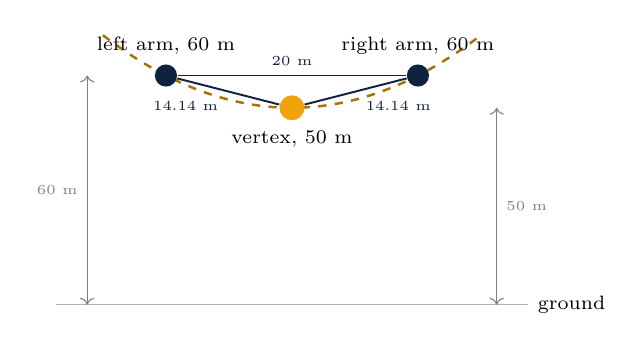
\begin{tikzpicture}[scale=1.0]
  \draw[gray!60] (-3,0)--(3,0) node[right,font=\scriptsize,black]{ground};
  \draw[amber!70!black,dashed,line width=0.9pt,domain=-2.4:2.4,samples=50] plot (\x,{2.5+0.16*\x*\x});
  \node[leader,label={[font=\scriptsize]below:vertex, 50 m}] (v) at (0,2.5) {};
  \node[drone,minimum size=8pt,label={[font=\scriptsize]above:left arm, 60 m}] (a) at (-1.6,2.91) {};
  \node[drone,minimum size=8pt,label={[font=\scriptsize]above:right arm, 60 m}] (b) at (1.6,2.91) {};
  \draw[link] (v)--node[below left,font=\tiny]{14.14 m}(a);
  \draw[link] (v)--node[below right,font=\tiny]{14.14 m}(b);
  \draw[link] (a)--node[above,font=\tiny]{20 m}(b);
  \draw[<->,gray] (2.6,0)--(2.6,2.5) node[midway,right,font=\tiny]{50 m};
  \draw[<->,gray] (-2.6,0)--(-2.6,2.91) node[midway,left,font=\tiny]{60 m};
\end{tikzpicture}
\caption[The parabola formation seen from behind]{The parabola formation seen from behind. All
three pairs keep a direct link (full mesh), and every link is within the 100\,m communication
range.}
\label{fig:parabola}
\end{figure}

\noindent At run time the vertex corridor is split into legs of at most 200\,m, and the arms are
derived parallel at $\pm10$\,m. All three drones fly one shared timetable, so they arrive at each
waypoint together even though the vertex has 10\,m less to climb.

\needspace{6\baselineskip}
\paragraph{Action order} ENHSP applies the actions in this order:
\actionflow{pre-flight-check, takeoff, climb (each drone) \then establish-comm-link (six times)
and confirm-swarm-comm (three times) \then take-parabola-slot (each drone) \then
establish-parabola-formation \then [formation-cruise \then hold-parabola-shape] for every leg
\then complete-parabola-mission}
A complete solved plan is shown in Section~\ref{sec:sampleplan}.

\screenshot{parabola.png}{Parabola formation in the simulator}{Parabola formation in the
simulator: the vertex route and the two arm routes beside it.}{fig:out-parabola}

%% ---------------------------------------------------------------------
\section{Figure-Eight Train Formation}\label{sec:plan-fig8}
\paragraph{What the mission does}
The swarm flies a figure-eight in the air as a \emph{train}: one drone behind another along the
curve, 10\,m apart. The operator makes four clicks: a base, then the left end, the crossing point
and the right end of the eight. Each lobe is half a lemniscate of Gerono from the crossing to its
clicked end, so the lobes cross at right angles and may differ in size (Figure~\ref{fig:fig8}).
The drones fly from the base to the crossing along a Dubins path (turn radius at least 25\,m),
fly the requested number of laps, and return to their own landing pads.

\glancebox{At a glance: figure-eight train}{
Map input & base, left end, crossing, right end; number of laps \\
Drones & 2 up to the capacity of the drawn eight (\maxFig{} on a typical eight) \\
Neighbours per drone & 1 or 2 -- the drone in front and the drone behind \\
ENHSP plans & the leader's lap and the lap count \\
Special feature & capacity rule checked in PDDL; laps counted, not unrolled \\}

\paragraph{Communication}
Like the carriages of a train, each drone talks only to the drone directly in front of it and
the drone directly behind it. The leader and the last drone have one neighbour each
(Figure~\ref{fig:comm-fig8}).

\begin{figure}[H]
\centering
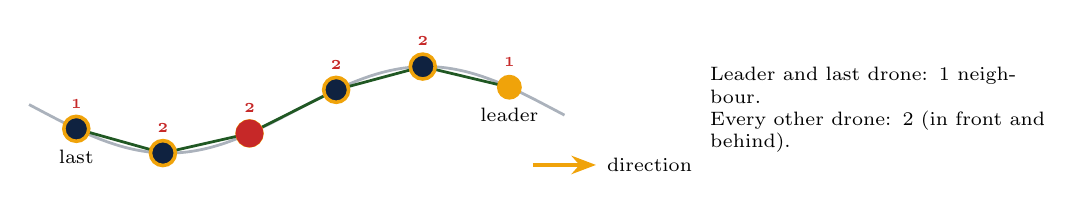
\begin{tikzpicture}
  \draw[navy!35,line width=1pt,domain=-3.4:3.4,samples=60,smooth] plot (\x,{0.55*sin(\x*55)});
  \foreach \i/\x in {0/2.7,1/1.6,2/0.5,3/-0.6,4/-1.7,5/-2.8}
    \coordinate (t\i) at (\x,{0.55*sin(\x*55)});
  \foreach \a/\b in {0/1,1/2,2/3,3/4,4/5} \draw[comm] (t\a)--(t\b);
  \foreach \i in {1,2,3,4,5} \node[nbr] at (t\i) {};
  \node[leader] at (t0) {};
  \node[focus] at (t3) {};
  \foreach \i/\n in {0/1,1/2,2/2,3/2,4/2,5/1} \node[cnt] at ($(t\i)+(0,0.32)$) {\n};
  \node[font=\scriptsize,below=4pt] at (t0) {leader};
  \node[font=\scriptsize,below=4pt] at (t5) {last};
  \draw[amber,line width=1.3pt,-{Stealth}] (3.0,-0.7)--(3.8,-0.7) node[right,font=\scriptsize,black]{direction};
  \node[note] at (7.4,0.0) {Leader and last drone: 1 neighbour.\\Every other drone: 2 (in front
    and behind).};
\end{tikzpicture}
\caption[Communication in the figure-eight train]{Communication in the figure-eight train: each
drone talks to the drone in front and the drone behind.}
\label{fig:comm-fig8}
\end{figure}

\noindent In PDDL the chain is the \code{train-neighbor} relation. Forming the train needs every
follower to have \code{neighbor-comm-ok}, and also checks the capacity rule:

\begin{lstlisting}
;; problem: leader <-> first follower (the chain is extended for every extra drone)
(train-neighbor drone-lead drone-f1)
(train-neighbor drone-f1 drone-lead)
(neighbor-comm-ok drone-lead)
(neighbor-comm-ok drone-f1)

;; domain: the train is formed only if it fits the eight and everyone is in contact
(:action establish-figure8-formation
    :parameters (?lead - drone ?l - location)
    :precondition (and (train-leader ?lead) (in-formation ?lead) (at ?lead ?l)
                       (at-cruise-altitude ?lead) (neighbor-comm-ok ?lead)
                       (>= (crossing-gap) (crossing-clearance))
                       (forall (?f - drone)
                           (or (not (train-follower ?f))
                               (and (in-formation ?f) (at ?f ?l)
                                    (at-cruise-altitude ?f) (neighbor-comm-ok ?f)))))
    :effect (and (figure8-established) (formation-at ?l) (train-closed)))
\end{lstlisting}

\paragraph{Important PDDL}
The leader's lap is planned through nine key waypoints with \code{formation-cruise}, and
\code{follow-leader} moves the followers after every leg. Laps are counted with a number, so
that 20 laps do not make the plan 20 times longer:

\begin{lstlisting}
(:action start-next-lap
  :parameters (?lead - drone ?dest - location ?start - location)
  :precondition (and (lap-end ?dest) (lap-start ?start) (figure8-established)
                     (train-closed) (formation-at ?dest) (train-leader ?lead)
                     (at ?lead ?dest) (< (+ (laps-completed) 1) (laps-required)))
  :effect (and (not (formation-at ?dest)) (formation-at ?start)
               (not (at ?lead ?dest)) (at ?lead ?start)
               (increase (laps-completed) 1)))
\end{lstlisting}

\noindent\textbf{Capacity.} The only place the train can meet itself is the crossing. The train
length $(N-1)\times10$\,m plus 14.1\,m of crossing clearance must therefore fit inside the
smaller lobe. This rule is checked in the GUI before planning, again in the plan worker, and
inside PDDL itself (the \code{crossing-gap} condition above), so ENHSP refuses an over-full
eight.

\begin{figure}[H]
\centering
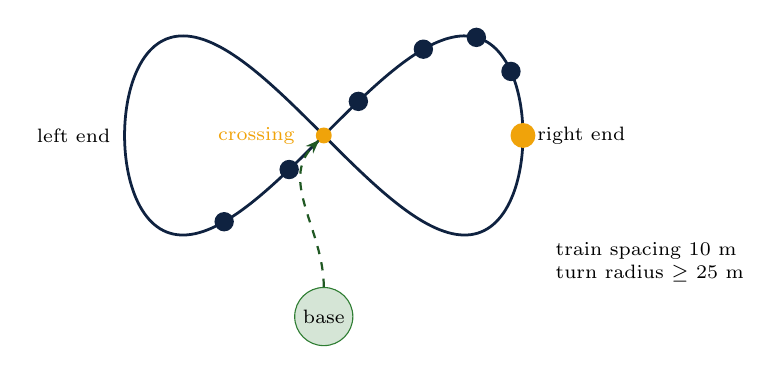
\begin{tikzpicture}[scale=1.15]
  \draw[navy,line width=1.0pt,domain=0:360,samples=120,smooth]
     plot ({2.2*cos(\x)},{1.1*sin(2*\x)});
  \foreach \t in {20,40,60,80,100,120} \node[drone] at ({2.2*cos(\t)},{1.1*sin(2*\t)}) {};
  \node[leader] at ({2.2*cos(0)},{1.1*sin(0)}) {};
  \fill[amber] (0,0) circle (2.5pt) node[left=7pt,font=\scriptsize]{crossing};
  \node[font=\scriptsize,right] at (2.25,0) {right end};
  \node[font=\scriptsize,left] at (-2.25,0) {left end};
  \node[circle,draw=okgreen,fill=okgreen!20,inner sep=2pt,font=\scriptsize] (base) at (0,-2.0) {base};
  \draw[darr,okgreen!70!black] (base) to[out=90,in=-135] (-0.05,-0.05);
  \node[font=\scriptsize,align=left] at (3.6,-1.4) {train spacing 10 m\\turn radius $\geq$ 25 m};
\end{tikzpicture}
\caption[The figure-eight train]{The figure-eight train. The leader (amber) and followers fly the
same path one spacing apart; the base leg joins the eight tangentially at the crossing.}
\label{fig:fig8}
\end{figure}

\needspace{6\baselineskip}
\paragraph{Action order} ENHSP applies the actions in this order:
\actionflow{pre-flight-check, takeoff, climb (each drone) \then take-train-slot (each drone)
\then establish-figure8-formation \then fly-to-pattern \then [formation-cruise \then
follow-leader] for the nine legs of a lap \then start-next-lap (repeat the lap) \then
finish-laps \then return-to-base \then complete-figure8-mission}

\screenshot{figure8.png}{Figure-eight train in the simulator}{Figure-eight train in the
simulator: the drones flying the eight one behind another.}{fig:out-fig8}

%% ---------------------------------------------------------------------
\section{Star Drone Show}\label{sec:plan-star}
\paragraph{What the mission does}
The operator picks a source for take-off and a destination for the show. Drones leave their
source pads one by one, with a 30\,m gap along the shared corridor, and take their places on a
circle around the destination. For each lap they form a star, return to the circle, spin the
circle once, form the star again, spin the star and return to the circle. They then return one
by one and land on their own source pads (Figure~\ref{fig:shows}a). Six or seven drones make a
3-pointed star, eight or nine a 4-pointed star, and ten or more a 5-pointed star. The destination
must be far enough from the source to leave room for the pads, corridor and show.

\glancebox{At a glance: star drone show}{
Map input & source and show destination; number of laps and show speed \\
Drones & 6 to \maxStar{} \\
Neighbours per drone & 2 -- the drones on either side round the circle \\
ENHSP plans & departure order, show phases, return order and landing \\
Special feature & drones keep their order round the centre, so shape changes never cross \\}

\paragraph{Communication}
The drones stand in a ring. Each drone talks to the two drones on either side of it round the
circle, so every drone has exactly two neighbours (Figure~\ref{fig:comm-star}).

\begin{figure}[H]
\centering
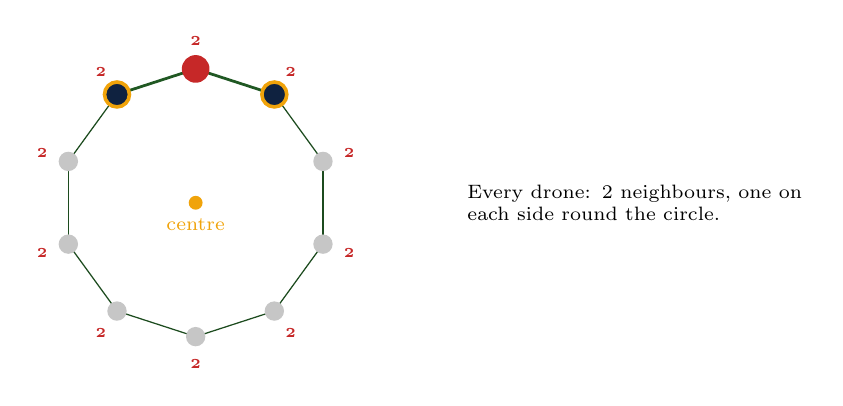
\begin{tikzpicture}
  \foreach \k in {0,...,9} \coordinate (r\k) at ({90+\k*36}:1.7);
  \foreach \k in {0,...,9} {
    \pgfmathtruncatemacro{\nx}{mod(\k+1,10)}
    \draw[commthin] (r\k)--(r\nx);
  }
  \draw[comm] (r0)--(r1); \draw[comm] (r0)--(r9);
  \foreach \k in {2,...,8} \node[other] at (r\k) {};
  \node[nbr] at (r1) {}; \node[nbr] at (r9) {};
  \node[focus] at (r0) {};
  \foreach \k in {0,...,9} \node[cnt] at ({90+\k*36}:2.05) {2};
  \fill[amber] (0,0) circle (2.5pt) node[below=2pt,font=\scriptsize]{centre};
  \node[note] at (5.6,0) {Every drone: 2 neighbours, one on each side round the circle.};
\end{tikzpicture}
\caption[Communication in the star show]{Communication in the star show: a ring in which every
drone talks to its two neighbours.}
\label{fig:comm-star}
\end{figure}

\noindent In PDDL this is the \code{ring-neighbor} relation. The show can only start when every
drone has climbed and has \code{neighbor-comm-ok}:

\begin{lstlisting}
;; problem: one ring pair of the template (the full ring is built on expansion)
(ring-neighbor drone-lead drone-m1)
(ring-neighbor drone-m1 drone-lead)
(neighbor-comm-ok drone-lead)
(neighbor-comm-ok drone-m1)

;; domain: the circle is formed only when every member is up and in contact
(:action form-circle
        :parameters
            (?lead - drone)
        :precondition
            (and
                (formation-leader ?lead)
                (neighbor-comm-ok ?lead)
                (not (show-started))
                (forall (?m - drone)
                    (or
                        (not (has-slot ?m))
                        (and
                            (in-slot ?m)
                            (neighbor-comm-ok ?m)
                        )
                    )
                )
            )
        :effect
            (and
                (show-started)
                (circle-formed)
            )
    )
\end{lstlisting}

\paragraph{Important PDDL}
Each phase of the show is one action that switches the current shape, for example
\code{form-star}, which turns the circle into a star at the start of a lap:

\begin{lstlisting}
(:action form-star
    :parameters (?lead - drone)
    :precondition (and (formation-leader ?lead) (circle-formed) (not (lap-started))
                       (< (laps-completed) (laps-required))
                       (gps-ok ?lead) (communication-ok ?lead))
    :effect (and (not (circle-formed)) (star-formed) (lap-started)))
\end{lstlisting}

\noindent The plan worker checks that ENHSP returns exactly the expected sequence. Every drone
keeps the same order round the centre in the circle and in the star, so shape changes never
cross paths; the show is sized so that all drones are at least 10\,m apart in each shape and at
least 9\,m apart during transitions.

\needspace{6\baselineskip}
\paragraph{Action order} ENHSP applies the actions in this order:
\actionflow{pre-flight-check, takeoff, climb (each drone) \then fly-to-formation (in order) \then form-circle \then [form-star \then
form-circle-in-lap \then spin-circle \then form-star-again \then spin-star \then close-lap] for
every lap \then end-show \then return-to-source and land (in order) \then complete-show}

\screenshot{star.png}{Star show in the simulator}{Star drone show in the simulator: the drones in
the star shape round the picked centre.}{fig:out-star}

%% ---------------------------------------------------------------------
\section{Planetary Orbit Show}\label{sec:plan-planets}
\paragraph{What the mission does}
The operator picks a source for take-off and a destination as the sun. Drones leave the source
one by one, 30\,m apart on the corridor, and join their orbits from the innermost outward.
For drone index $k=0,1,\ldots,N-1$, the nominal orbit radius is $50+10k$\,m: 50 to 120\,m for
eight drones. Neighbouring orbits turn in opposite directions (Figure~\ref{fig:shows}b).
Every drone uses the same angular speed, so the outer drones fly faster. The drones turning
each way stay on one straight line out from the sun. One lap is one full turn for every drone;
both lines meet on the starting line at the end of each lap. Drones return one by one, outermost
first, and land on their own source pads. Moves start and stop smoothly over five clock seconds.
The destination must be at least the outermost orbit radius plus 50\,m from the source.

\glancebox{At a glance: planetary orbit show}{
Map input & source and destination (the sun); laps and show speed \\
Drones & 2 to \maxPlanets{} (one per planet) \\
Neighbours per drone & 1 or 2 -- the drones on the next orbit in and the next orbit out \\
ENHSP plans & departure order, entering orbits, laps, return and landing \\
Special feature & neighbouring orbits must turn in opposite directions \\}

\paragraph{Communication}
Each drone talks to the drones on the orbits just inside and just outside its own. The innermost
and outermost drones therefore have one neighbour, and the others two
(Figure~\ref{fig:comm-planets}).

\begin{figure}[H]
\centering
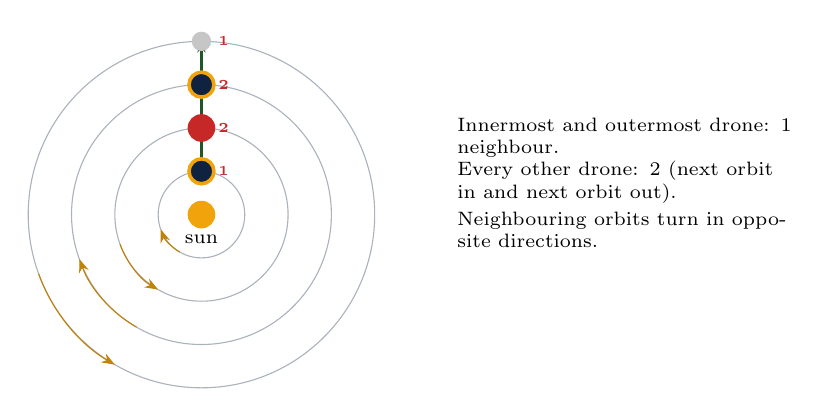
\begin{tikzpicture}
  \fill[amber] (0,0) circle (5pt);
  \node[font=\scriptsize,below=4pt] at (0,0) {sun};
  \foreach \k in {1,2,3,4} \draw[navy!35] (0,0) circle (\k*0.55);
  \foreach \k in {1,2,3,4} \coordinate (p\k) at (90:\k*0.55);
  \draw[comm] (p1)--(p2); \draw[comm] (p2)--(p3); \draw[comm] (p3)--(p4);
  \node[nbr] at (p1) {}; \node[focus] at (p2) {}; \node[nbr] at (p3) {}; \node[other] at (p4) {};
  \foreach \k/\n in {1/1,2/2,3/2,4/1} \node[cnt] at ($(p\k)+(0.28,0)$) {\n};
  \foreach \k/\dir in {1/-1,2/1,3/-1,4/1} {
    \ifnum\dir=1
      \draw[-{Stealth},amber!80!black] (200:\k*0.55) arc (200:240:\k*0.55);
    \else
      \draw[-{Stealth},amber!80!black] (240:\k*0.55) arc (240:200:\k*0.55);
    \fi
  }
  \node[note] at (5.4,0.4) {Innermost and outermost drone: 1 neighbour.\\Every other drone: 2
    (next orbit in and next orbit out).\\[2pt]Neighbouring orbits turn in opposite directions.};
\end{tikzpicture}
\caption[Communication in the planetary show]{Communication in the planetary show: each drone
talks to the drones on the neighbouring orbits.}
\label{fig:comm-planets}
\end{figure}

\noindent In PDDL this is the \code{orbit-neighbor} relation. The drones may enter their orbits
only when every drone is up and in contact, and only if every pair of orbit neighbours turns in
opposite directions:

\begin{lstlisting}
;; problem: the two template planets are orbit neighbours
(orbit-neighbor drone-mercury drone-venus)
(orbit-neighbor drone-venus drone-mercury)
(neighbor-comm-ok drone-mercury)
(neighbor-comm-ok drone-venus)

;; domain: enter the orbits only if everyone is in contact and neighbours turn opposite ways
(:action enter-orbits
        :parameters
            (?lead - drone)
        :precondition
            (and
                (formation-leader ?lead)
                (neighbor-comm-ok ?lead)
                (not (orbits-entered))
                (forall (?m - drone)
                    (or
                        (not (has-orbit ?m))
                        (and
                            (on-orbit ?m)
                            (neighbor-comm-ok ?m)
                        )
                    )
                )
                (forall (?a - drone ?b - drone)
                    (or
                        (not (orbit-neighbor ?a ?b))
                        (and (orbits-clockwise ?a) (orbits-anticlockwise ?b))
                        (and (orbits-anticlockwise ?a) (orbits-clockwise ?b))
                    )
                )
            )
        :effect
            (orbits-entered)
    )
\end{lstlisting}

\paragraph{Important PDDL}
After the orbits are entered, one \code{fly-lap} action follows per lap, counted by
\code{laps-completed}, and then \code{end-show}, ordered returns, \code{land} and \code{complete-planets}:

\begin{lstlisting}
(:action fly-lap
    :parameters (?lead - drone)
    :precondition (and (formation-leader ?lead) (orbits-entered)
                       (< (laps-completed) (laps-required))
                       (gps-ok ?lead) (communication-ok ?lead))
    :effect (increase (laps-completed) 1))
\end{lstlisting}

\needspace{6\baselineskip}
\paragraph{Action order} ENHSP applies the actions in this order:
\actionflow{pre-flight-check, takeoff, climb (each drone) \then fly-to-orbit (in order) \then enter-orbits \then fly-lap (once
per lap) \then end-show \then return-to-source and land (in order) \then complete-planets}

\begin{figure}[H]
\centering
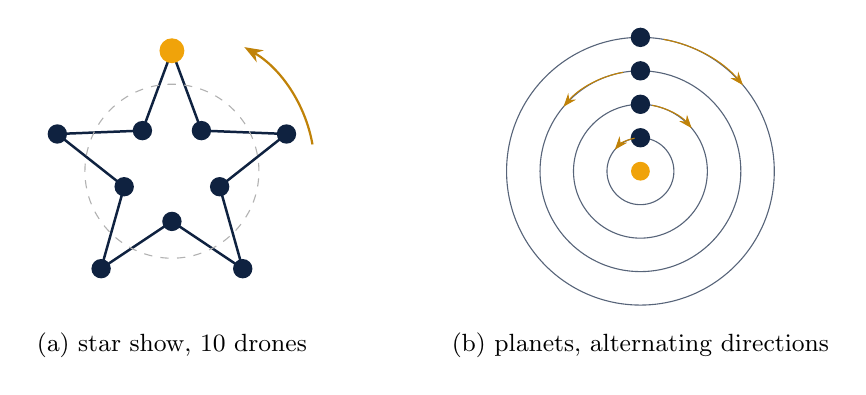
\begin{tikzpicture}[scale=0.85]
  \begin{scope}
    \foreach \k in {0,...,9} {
      \pgfmathsetmacro{\r}{ifthenelse(mod(\k,2)==0,1.8,0.75)}
      \coordinate (s\k) at ({90+\k*36}:\r);
    }
    \draw[navy,line width=0.9pt] (s0)--(s1)--(s2)--(s3)--(s4)--(s5)--(s6)--(s7)--(s8)--(s9)--cycle;
    \draw[gray!60,dashed] (0,0) circle (1.3);
    \foreach \k in {0,...,9} \node[drone] at (s\k) {};
    \node[leader] at (s0) {};
    \draw[amber!80!black,-{Stealth},line width=0.8pt] (2.1,0.4) arc (10:60:2.1);
    \node[font=\small] at (0,-2.6) {(a) star show, 10 drones};
  \end{scope}
  \begin{scope}[xshift=7cm]
    \fill[amber] (0,0) circle (4pt);
    \foreach \k/\dir in {1/1,2/-1,3/1,4/-1} {
      \draw[navy!70] (0,0) circle (\k*0.5);
      \node[drone] at (90:\k*0.5) {};
      \ifnum\dir=1
        \draw[-{Stealth},amber!80!black] (100:\k*0.5) arc (100:140:\k*0.5);
      \else
        \draw[-{Stealth},amber!80!black] (80:\k*0.5) arc (80:40:\k*0.5);
      \fi
    }
    \node[font=\small] at (0,-2.6) {(b) planets, alternating directions};
  \end{scope}
\end{tikzpicture}
\caption[Shape-changing shows: star and planets]{Shape-changing shows. Both are flown against a
shared timetable so that every phase starts and ends together for all drones.}
\label{fig:shows}
\end{figure}

\screenshot{planets.png}{Planetary show in the simulator}{Planetary orbit show in the simulator:
one drone per orbit round the picked centre.}{fig:out-planets}

%% ---------------------------------------------------------------------
\section{Road Inspection}\label{sec:plan-inspect}
\paragraph{What the mission does}
The operator clicks a source and a destination on a road. One drone takes off at the source,
follows the road's exact path to the destination, flies the same road back and lands at the
source. The road geometry comes from an OSRM routing server on OpenStreetMap data. If no road
route exists, a click is more than 30\,m from any road, or the two points are less than 20\,m
apart along the road, the plan fails before anything flies.

\glancebox{At a glance: road inspection}{
Map input & two points on a road \\
Drones & 1 \\
Neighbours per drone & none -- ground station link only \\
ENHSP plans & every road segment, out and back \\
Special feature & road geometry from OSRM; at most 12 segments \\}

\paragraph{Communication}
There is only one drone, so it has no neighbours. It keeps its link to the ground station during
the whole inspection (Figure~\ref{fig:comm-inspect}).

\begin{figure}[H]
\centering
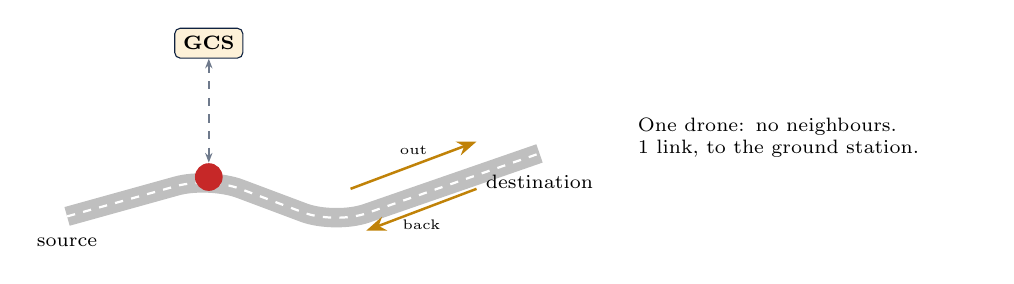
\begin{tikzpicture}
  \draw[gray!50,line width=7pt,rounded corners=12pt] (-3,-0.6)--(-1.2,-0.1)--(0.4,-0.7)--(3,0.2);
  \draw[white,line width=0.8pt,dashed,rounded corners=12pt] (-3,-0.6)--(-1.2,-0.1)--(0.4,-0.7)--(3,0.2);
  \node[focus] (d) at (-1.2,-0.1) {};
  \node[gcs] (g) at (-1.2,1.6) {GCS};
  \draw[glink] (g)--(d);
  \node[font=\scriptsize,below] at (-3,-0.75) {source};
  \node[font=\scriptsize,below] at (3,0.05) {destination};
  \draw[amber!80!black,-{Stealth},line width=0.9pt] (0.6,-0.25)--(2.2,0.35) node[midway,above,font=\tiny,black]{out};
  \draw[amber!80!black,-{Stealth},line width=0.9pt] (2.2,-0.25)--(0.8,-0.78) node[midway,below,font=\tiny,black]{back};
  \node[note] at (6.4,0.4) {One drone: no neighbours.\\1 link, to the ground station.};
\end{tikzpicture}
\caption[Communication in road inspection]{Communication in road inspection: a single drone
linked to the ground station.}
\label{fig:comm-inspect}
\end{figure}

\noindent As in travel, the ground link is the flag \code{communication-ok}, which every
inspection step requires.

\paragraph{Important PDDL}
The road is split into at most 12 segments, each with its own length and energy. Each segment is
inspected in order, and only if the battery covers it:

\begin{lstlisting}
(:action inspect-segment
    :parameters (?d - drone ?from - location ?to - location)
    :precondition (and (inspector ?d) (road-segment ?from ?to)
                       (not (segment-inspected ?from ?to)) (not (road-inspected))
                       (at ?d ?from) (at-cruise-altitude ?d)
                       (gps-ok ?d) (communication-ok ?d) (drone-healthy ?d)
                       (> (battery ?d) (energy-required ?from ?to)))
    :effect (and (not (at ?d ?from)) (at ?d ?to) (segment-inspected ?from ?to)
                 (increase (segments-inspected) 1)
                 (decrease (battery ?d) (energy-required ?from ?to))))
\end{lstlisting}

\needspace{6\baselineskip}
\paragraph{Action order} ENHSP applies the actions in this order:
\actionflow{pre-flight-check \then takeoff \then climb-to-cruise-altitude \then inspect-segment
(each segment in order) \then finish-inspection \then return-along-road (each segment back)
\then land-at-source}

\screenshot{inspect.png}{Road inspection in the simulator}{Road inspection in the simulator: the
drone's route following the real road between the two clicked points.}{fig:out-inspect}

%% ---------------------------------------------------------------------

\section{Battery-Aware Travel}\label{sec:plan-battery}
\paragraph{What the mission does}
One drone flies from the source to the destination. The operator also marks five charging
stations before the route is chosen. If the current battery can cover the direct trip and its
margin, the drone flies straight to the destination. Otherwise, the planner chooses a route
through reachable stations. Other selected drones stay on the ground.

\glancebox{At a glance: battery-aware travel}{
Map input & source, destination and five charging stations \\
Drones & 1, the first selected drone \\
Neighbours per drone & none; ground-station link only \\
ENHSP plans & reachable hops and charging stops, using optimal search \\
Special feature & charge only for the next hop plus a 10\,\% margin \\}

\paragraph{Communication}
The drone sends its position and battery state to the ground station. After each station
landing, the ground station sends a charge command. It sends the next flight only after the
required charge is reached. No drone-to-drone link is needed.

\paragraph{Important PDDL}
Each hop includes take-off, climb, flight and descent. Its energy estimate uses the simulated
current draw, battery capacity, flight speed and height, with ten extra seconds for transitions.
At a station, \code{charge-battery} sets the battery to the next hop's energy plus ten percentage
points. The \code{charged-for} fact ties that charge to that specific hop. Take-off is blocked
until charging is complete. A target above 100\,\% is not allowed. The route metric is metres
flown plus one per station landing; an independent shortest-path check checks the chosen route.
The old rule of charging to full with a 25\,\% reserve is no longer used.

\begin{lstlisting}
(:action charge-battery
        :parameters
            (?d - drone
             ?l - location
             ?to - location)
        :precondition
            (and
                (at ?d ?l)
                (charging-station ?l)
                (landed ?d)
                (needs-charge ?d)
                (hop ?l ?to)
                (< (battery ?d) (+ (hop-energy ?l ?to) (charge-margin ?d)))
                (<= (+ (hop-energy ?l ?to) (charge-margin ?d)) (max-battery ?d))
            )
        :effect
            (and
                (not (needs-charge ?d))
                (charged-for ?d ?l ?to)
                (assign (battery ?d) (+ (hop-energy ?l ?to) (charge-margin ?d)))
            )
    )
\end{lstlisting}

\paragraph{Action order} The actions follow this order:
\actionflow{pre-flight-check \then take-off \then fly-hop \then [land-at-station \then
charge-battery \then take-off \then fly-hop] as needed \then land-at-destination \then complete-mission}

\paragraph{Output}
The map shows the chosen route and the stations it uses. The drone lands and charges at each
chosen station, then continues. A planned charging hop can land near 10\,\% battery, so the
ordinary 20\,\% warning is skipped for this mission; the critical 5\,\% safeguard still applies.
If no chain of stations is reachable, the operator must place the stations again.

\section{Formula-4: Dynamic Position Swaps}\label{sec:plan-formula4}
\paragraph{What the mission does}
Four drones fly in two lanes from source to destination. Each lane has a front and a back drone.
The front drone slows and dips to 50\,m. The back drone speeds up, climbs to 60\,m and passes it.
They repeat these swaps along the route and land in their own destination slots.

\glancebox{At a glance: Formula-4}{
Map input & source and destination \\
Drones & 4, the first four selected drones \\
Neighbours per drone & no drone-to-drone messages \\
ENHSP plans & formula checks and each drone's swaps, arrival and landing \\
Special feature & safe passing from a position formula and one shared clock \\}

\paragraph{Communication}
Each drone follows its own timed track. It needs its starting slot and the shared clock from
the ground station. It does not need the current positions of the other drones.

\paragraph{Important PDDL}
Let $x$ be distance along the route, $y$ distance across it and $z$ height. The front/back sign
is $f=+1/-1$ and the left/right sign is $l=+1/-1$. At shared clock time $\tau$,
\[
 x=V\tau+f\frac D2\cos(\omega\tau),\qquad
 y=l\left(\frac W2+f\frac B2\sin(\omega\tau)\right),\qquad
 z=Z_0-fA\sin(\omega\tau).
\]
Here $D=W=20$\,m, $B=6$\,m, $Z_0=55$\,m and $A=5$\,m. The speed $V$ is 6 metres per clock
second. The turn rate gives an even number of swaps, so drones finish in their starting slot
order. In the same lane, the distance is at least
$\min(D,\sqrt{B^2+4A^2})=11.66$\,m; across a line it is at least $W-B=14$\,m.
The \code{check-formula} action checks these bounds and the speed limits before take-off.
These are bounds for the planned formula; actual flight also depends on tracking that formula.

\paragraph{Action order} The actions follow this order:
\actionflow{check-formula \then take-off (each drone) \then slow-and-dip / speed-up-and-climb
(alternating for each drone) \then arrive \then land}

\paragraph{Output}
The simulator shows repeated passes, with the passing drone above the slower drone. Heights
change throughout the flight. The worker checks each drone's action sequence before sending
the timed tracks. Show speed changes how fast the shared clock runs.

\section{Formation-Circle: A Rotating Vertical Circle}\label{sec:plan-circle}
\paragraph{What the mission does}
Four drones form a vertical circle across the route. They start at the bottom, left, top and
right, at heights of 40, 50, 60 and 50\,m. The circle turns while moving toward the destination.
Each drone moves bottom to left to top to right, so its flight path is a spiral.

\glancebox{At a glance: Formation-Circle}{
Map input & source and destination \\
Drones & 4, the first four selected drones \\
Neighbours per drone & no drone-to-drone messages \\
ENHSP plans & formula checks, joining, quarter turns, leaving and landing \\
Special feature & a rotating vertical circle with separate take-off and landing pads \\}

\paragraph{Communication}
As in Formula-4, each drone uses its own starting place and the shared ground-station clock.
No drone needs to ask a neighbour for its position.

\paragraph{Important PDDL}
With radius $R=10$\,m, centre height $Z_0=50$\,m and starting angle $a_{i0}$, the main flight is
\[
 a_i=a_{i0}+\omega(\tau-T_j),\qquad
 x_i=V\tau,\qquad y_i=R\sin(a_i),\qquad z_i=Z_0-R\cos(a_i).
\]
The starting angles differ by a quarter turn. Neighbours stay $R\sqrt{2}=14.14$\,m apart in
the formula, and opposite drones stay $2R=20$\,m apart. The \code{check-formula} action checks
these gaps, the pad spacing, speed and lowest height. The circle makes a whole number of turns.

The top and bottom drones cannot take off from the same ground point. They therefore start on
separate pads in a diamond. The diamond closes into the circle over the first 40\,m and opens
again over the last 40\,m. Each drone then lands on its own destination pad. These joins also
keep the planned separation; actual tracking can give slightly different measured gaps.

\paragraph{Action order} The actions follow this order:
\actionflow{check-formula \then take-off (each drone) \then join-circle \then turn-quarter
(four per full turn, for each drone) \then leave-circle \then land}

\paragraph{Output}
The simulator shows a circle that moves forward while turning, with each drone changing height
and side. Long timed tracks are split into smaller UDP messages and joined again at the drone.
Both formula plans have a 9000-point track limit, so their maximum route length depends on how
many track points the movement needs.

\section{Task Allocation with a Standby Drone}\label{sec:plan-task}
\paragraph{What the model does}
Four capable drones start at the source. One drone takes responsibility and starts the task.
The others wait. If the active drone develops a recoverable problem, it reserves a capable
standby drone. The replacement takes off; while both drones are airborne and their radios work,
the old drone shares the mission data and transfers the task. The replacement can repeat this
process if it later develops a problem.

\glancebox{At a glance: task allocation model}{
Map input & source and destination, at least 30\,m apart \\
Drones & exactly 4 selected; one active owner at a time \\
Communication & working radios on both drones during the airborne handoff \\
Planner models & task ownership, standby launch, data transfer and completion \\
Current status & PDDL plan plus a runtime controller in the drone-thread backend \\}

\paragraph{Important PDDL}
The \code{responsible} and \code{mission-data} facts identify the active owner. Reserving a
standby removes it from the available pool. The handoff removes the old drone's mission data
and marks it retired. Arrival completes the task and sets \code{mission-finished}; every action
requires the mission to remain unfinished, so no replacement can launch after completion.

\begin{lstlisting}
(:action share-data-and-transfer-task
        :parameters (?old - drone ?new - drone ?from - location ?to - location)
        :precondition (and
            (not (mission-finished)) (replacement-launched ?old ?new)
            (failed ?old) (mission-data ?old)
            (airborne ?old) (airborne ?new)
            (en-route ?old ?from ?to) (en-route ?new ?from ?to)
            (communication-ok ?old) (communication-ok ?new))
        :effect (and
            (not (replacement-launched ?old ?new))
            (mission-data ?new) (responsible ?new)
            (not (mission-data ?old)) (retired ?old))
    )
\end{lstlisting}

\paragraph{Action order} The actions follow this order:
\actionflow{start-mission \then [detect-problem \then notify-capable-drone \then
launch-replacement \then share-data-and-transfer-task] if needed \then travel-to-destination}

\paragraph{Simulator execution}
The plan service checks the four drone profiles, removes capability facts for drones that
cannot fly the route and asks ENHSP to choose an initial owner. All four drone threads start
at the source, but only the owner receives a flight command. The runtime controller watches
faults, GPS state and low battery. It picks an available standby with enough charge to fly
the whole route from the source. The standby climbs above 1\,m, receives the task data through
the ground station and reports that data back in its state. Only then does it become the owner;
the old drone receives a landing command. A failed or timed-out standby is retired and another
candidate is tried. Arrival closes allocation, so no further drone launches.

\paragraph{Limits}
The PDDL file describes a handoff with two airborne drones and working radios. Known
\code{will-fail} facts can let classical planning choose a healthy drone directly. Unexpected
faults are handled by the runtime controller; it does not rerun ENHSP for every handoff.
The controller relays stored task data rather than using a direct drone-to-drone transfer.
For communication loss or an unavailable drone, it can use its cached copy. This is a wider
runtime behaviour than the PDDL handoff alone describes. Emergency landing and actual fault
recovery still depend on the flight backend. No successful flight measurements for this new
task-allocation code were found in the checked status notes.


\section{Summary of the Plans}
Table~\ref{tab:plansummary} compares the fourteen simulator plans side by side.

\begin{table}[H]
\caption{Comparison of the mission plans}\label{tab:plansummary}
\small
\begin{tabularx}{\textwidth}{@{}lP{0.13\textwidth}P{0.13\textwidth}P{0.17\textwidth}Y@{}}
\toprule
\textbf{Plan} & \textbf{Drones} & \textbf{Neighbours per drone} & \textbf{What ENHSP plans} & \textbf{Special feature} \\
\midrule
Travel     & 1--\maxTravel & none & every drone's legs & full controller fault responses \\
Search     & 2--\maxSearch & none & one lane per drone & pairwise separation check \\
V          & 3--\maxV, odd & 1--2 & leader corridor & timed wing launch \\
Grid       & 4--\maxGrid & 2--4 & leader corridor & 4-neighbour links \\
Cube       & 8--\maxCube & up to 24 & leader corridor & layer-by-layer ascent \\
Parabola   & 3 & 2 & vertex corridor & range-checked link mesh, shape check \\
Figure-8   & 2--capacity & 1--2 & leader's lap & capacity rule, laps \\
Star       & 6--\maxStar & 2 & show phases & circle/star/spin sequence \\
Planets    & 2--\maxPlanets & 1--2 & show phases & opposite-direction orbits \\
Inspect    & 1 & none & road segments & OSRM road geometry \\
Battery-aware & 1 & none & hops and charges & next-hop charge plus margin \\
Formula-4 & 4 & none & swaps per drone & shared-clock passing \\
Circle & 4 & none & quarter turns & vertical rotating circle \\
Task allocation & 4 & handoff pair & initial owner and task completion & runtime standby replacement \\
\bottomrule
\end{tabularx}
\end{table}

%% =====================================================================
%%  CHAPTER 6  COMMUNICATION
%% =====================================================================
\chapter{Inter-Drone Communication}\label{ch:comm}
Formula-4 and Formation-Circle use a shared clock without drone-to-drone position messages.
Battery-aware travel uses only a ground-station link. The task-allocation PDDL model needs
working radios on both drones for a handoff; runtime data is relayed through the ground station. In the other plans, communication appears at two levels in the simulator. In the PDDL models it is a set of
conditions: a drone may only act if its links are up. At run time it is a real exchange of
messages between the ground station and the drones. This chapter explains both and how they
relate. The communication of each individual plan, with its own diagram and PDDL, is given in
the section of that plan in Chapter~\ref{ch:plans}.

\section{Communication in the PDDL Models}
Two flags carry communication state for every drone:
\begin{itemize}
  \item \code{communication-ok}: the link between the drone and the ground controller works;
  \item \code{neighbor-comm-ok}: the drone's links to its formation neighbours work.
\end{itemize}
Every action that moves a drone or changes the formation checks the relevant flags. A formation
cannot be established, cruise a leg or close up if any member has lost its neighbour links.
Each plan also declares \emph{who} must talk to whom, using a neighbour relation suited to its
shape (Table~\ref{tab:neighbors}, Figure~\ref{fig:topologies}).

\begin{table}[H]
\caption{Neighbour relations declared by each formation}\label{tab:neighbors}
\small
\begin{tabularx}{\textwidth}{@{}l>{\ttfamily\footnotesize}lY@{}}
\toprule
\textbf{Plan} & \textbf{\normalfont\small Relation} & \textbf{Who talks to whom} \\
\midrule
V formation & wing-neighbor   & leader with rank 1, then rank to rank along each wing (a chain) \\
Grid        & grid-neighbor   & up to 4 neighbours: front, back, left, right \\
Cube        & cube-neighbor   & up to 24 neighbours in the surrounding $3\times3\times3$ block,
excluding directly above and below \\
Parabola    & parabola-neighbor & all three pairs, in both directions (6 directed links) \\
Figure-8    & train-neighbor  & the drone in front and the drone behind \\
Star        & ring-neighbor   & the two drones on either side round the circle \\
Planets     & orbit-neighbor  & drones on adjacent orbits \\
\bottomrule
\end{tabularx}
\end{table}

\begin{figure}[H]
\centering
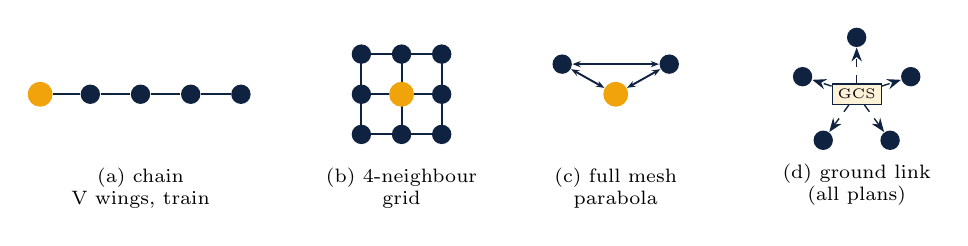
\begin{tikzpicture}[scale=0.85]
  % chain
  \begin{scope}
    \node[leader] (c0) at (0,0) {};
    \foreach \i in {1,...,4} \node[drone] (c\i) at (\i*0.75,0) {};
    \draw[link] (c0)--(c1)--(c2)--(c3)--(c4);
    \node[font=\scriptsize,align=center] at (1.5,-1.4) {(a) chain\\V wings, train};
  \end{scope}
  % grid 4-neighbour
  \begin{scope}[xshift=4.8cm,yshift=0.6cm]
    \foreach \r in {0,1,2} \foreach \c in {0,1,2} \coordinate (q\r\c) at (\c*0.6,-\r*0.6);
    \foreach \r in {0,1,2} \draw[link] (q\r0)--(q\r2);
    \foreach \c in {0,1,2} \draw[link] (q0\c)--(q2\c);
    \foreach \r in {0,1,2} \foreach \c in {0,1,2} \node[drone] at (q\r\c) {};
    \node[leader] at (q11) {};
    \node[font=\scriptsize,align=center] at (0.6,-2.0) {(b) 4-neighbour\\grid};
  \end{scope}
  % full mesh
  \begin{scope}[xshift=8.6cm]
    \node[leader] (m0) at (0,0) {};
    \node[drone] (m1) at (-0.8,0.45) {};
    \node[drone] (m2) at (0.8,0.45) {};
    \draw[link,{Stealth[length=3pt]}-{Stealth[length=3pt]}] (m0)--(m1);
    \draw[link,{Stealth[length=3pt]}-{Stealth[length=3pt]}] (m0)--(m2);
    \draw[link,{Stealth[length=3pt]}-{Stealth[length=3pt]}] (m1)--(m2);
    \node[font=\scriptsize,align=center] at (0,-1.4) {(c) full mesh\\parabola};
  \end{scope}
  % ground star
  \begin{scope}[xshift=12.2cm]
    \node[rectangle,draw=navy,fill=softamber,font=\tiny,inner sep=2pt] (g) at (0,0) {GCS};
    \foreach \a in {0,72,144,216,288} { \node[drone] (s\a) at (\a+90:0.85) {}; \draw[darr,line width=0.5pt] (g)--(s\a); }
    \node[font=\scriptsize,align=center] at (0,-1.35) {(d) ground link\\(all plans)};
  \end{scope}
\end{tikzpicture}
\caption[Communication topologies]{Communication topologies. (a)--(c) are drone-to-drone
relations declared in PDDL; (d) is the ground-controller link represented by
\code{communication-ok}.}
\label{fig:topologies}
\end{figure}

\section{The Range-Checked Link Model of the Parabola Plan}\label{sec:paracomm}
In most plans the links are summarised by the per-drone flag. The parabola plan models each
directed link explicitly (Section~\ref{sec:plan-parabola}). A link from $d_1$ to $d_2$ can be
established only when both drones are airborne at cruise altitude, both radios work, and the
straight-line distance between them is within the communication range of 100\,m. A drone
becomes \code{swarm-comm-ready} through \code{confirm-swarm-comm} once it has a link to every
one of its neighbours. Only then can it take its slot. During flight,
\code{hold-parabola-shape} requires every declared link to still be up, and if a drone loses its
neighbour links, \code{detect-neighbor-link-loss} removes all links to and from that drone, so
the shape cannot be re-formed until they are restored. A negative test with the range reduced to
15\,m (below the 20\,m arm-to-arm distance) correctly produced no plan. In the solved plan, the
six \code{establish-comm-link} actions and three \code{confirm-swarm-comm} actions appear right
after the climbs and before any slot is taken (Section~\ref{sec:sampleplan}).

\section{Run-Time Communication between Ground Station and Drones}
At run time each drone is an independent thread that owns its state. It can only be reached
through a command inbox and only reports through a telemetry callback. Over the network, the
ground station and drones use a simple JSON-over-UDP protocol, one datagram per message, designed
so that it can later be replaced by MAVLink. Every message carries the drone's MAVLink SYSID, so
one ground socket can address the whole swarm (Figure~\ref{fig:udp}).

\begin{figure}[H]
\centering
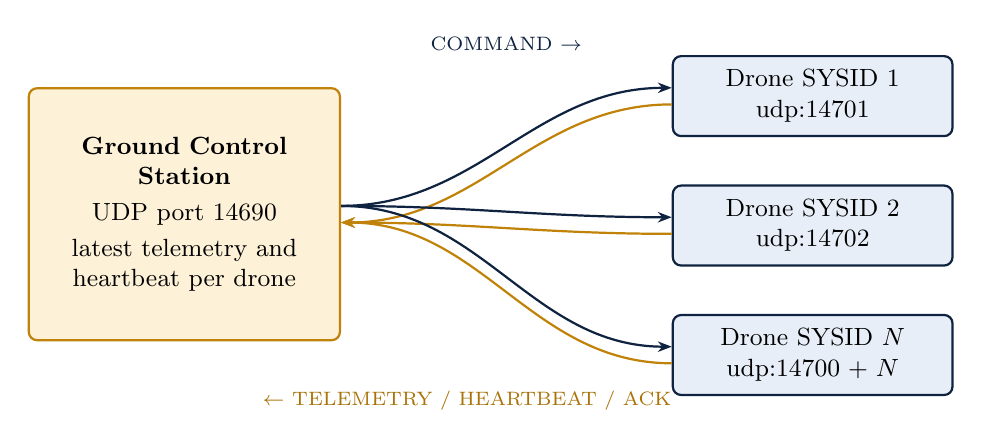
\begin{tikzpicture}[node distance=6mm]
  \node[abox,text width=3.6cm,minimum height=3.2cm] (gcs) {\textbf{Ground Control}\\\textbf{Station}\\[2pt]UDP port 14690\\[2pt]
     latest telemetry and heartbeat per drone};
  \node[box,right=4.2cm of gcs,yshift=1.5cm,text width=3.2cm] (d1) {Drone SYSID 1\\udp:14701};
  \node[box,below=6mm of d1,text width=3.2cm] (d2) {Drone SYSID 2\\udp:14702};
  \node[box,below=6mm of d2,text width=3.2cm] (dn) {Drone SYSID $N$\\udp:$14700+N$};
  \foreach \d in {d1,d2,dn} {
    \draw[arr] ([yshift=3pt]gcs.east) to[out=0,in=180] ([yshift=3pt]\d.west);
    \draw[arr,amber!80!black] ([yshift=-3pt]\d.west) to[out=180,in=0] ([yshift=-3pt]gcs.east);
  }
  \node[font=\scriptsize,navy,align=center] at ($(gcs.north east)!0.5!(d1.north west)+(0,0.35)$) {COMMAND $\rightarrow$};
  \node[font=\scriptsize,amber!70!black,align=center] at ($(gcs.south east)+(1.6,-0.75)$) {$\leftarrow$ TELEMETRY / HEARTBEAT / ACK};
\end{tikzpicture}
\caption[Run-time messaging between GCS and drones]{Run-time messaging. Commands are routed to a
port derived from each drone's SYSID; every drone reports back to one ground station socket.}
\label{fig:udp}
\end{figure}

\noindent Table~\ref{tab:commands} lists the commands. A drone sends a heartbeat every second
and telemetry every 0.5\,s. The ground station treats a drone as out of contact if no heartbeat
arrives for 3\,s. On the drone side, if nothing is heard from the ground for more than 5\,s the
drone marks its link \code{DEGRADED}, and after 10\,s \code{LOST}. Link loss is therefore
\emph{observed} from missing messages rather than assumed.

\begin{table}[H]
\caption{Commands of the ground-station-to-drone protocol}\label{tab:commands}
\small
\begin{tabularx}{\textwidth}{@{}>{\ttfamily\footnotesize}P{0.28\textwidth}Y@{}}
\toprule
\textbf{\normalfont\small Command} & \textbf{Purpose} \\
\midrule
NAVIGATE & The one mission operation: upload a whole route (approach, loop, laps, depart). \\
ARM, DISARM, TAKEOFF, LAND & Basic flight control. \\
HOLD, RESUME & Pause and continue the mission (used while the operator decides on a fault). \\
RETURN\_TO\_LAUNCH, ABORT & Fall back to the start point, or stop. \\
SET\_GPS & Fault injection: switch the drone's GPS fix off or on. \\
SET\_SPEED & Change cruise speed in flight. \\
TRAIN\_PACE & Formation keeping: the shared, time-stamped pace of the train or show clock. \\
PING, SHUTDOWN & Liveness check and stop the drone thread. \\
\bottomrule
\end{tabularx}
\end{table}

\section{On-Board Formation Keeping}\label{sec:pace}
\paragraph{The problem, in simple words}
In the figure-eight train every drone must stay 10\,m behind the drone in front. In the first
version, the ground station watched all the drones and sent each one ``speed up'' or ``slow
down'' commands. These commands always arrived a little late, two or three telemetry updates
after the gap was measured. By then the gap had already changed. A drone told to speed up was
still speeding up after it had caught up, then had to brake hard, and the drone behind copied
the same mistake even more strongly. Like a traffic jam on a highway, the error grew along the
train, and drones bunched together and even overtook each other.

\paragraph{The idea}
The ground station no longer steers each drone. It acts like the conductor of a band who only
keeps the beat. It broadcasts one shared message, \code{TRAIN\_PACE}, which says where the head
of the train should be, how fast it is moving and \emph{when} this was measured. Each drone does
the rest by itself, many times per second, using its own exact position.

\paragraph{What each drone does every tick}
\begin{enumerate}
  \item \textbf{Bring the pace up to date.} The drone moves the pace forward by the time since its
        time stamp. So even a message that arrives late gives the correct position for now.
  \item \textbf{Find its own target.} The drone subtracts its place in the train: drone number
        $k$ should be $k\times10$\,m behind the pace point.
  \item \textbf{Measure itself.} The drone measures how far it has really flown along its own
        route. This needs no message, so it has no delay.
  \item \textbf{Adjust its own speed.} If it is behind its target it speeds up a little; if it is
        ahead it slows down a little.
  \item \textbf{Stay safe.} If the drone in front is reported too close, the drone never speeds
        up, whatever its target says.
\end{enumerate}
The ground station keeps one extra job: if any drone falls far behind, it slows the pace, so the
whole train waits for that drone instead of leaving it behind.

\paragraph{Why it works}
The only thing that comes from the ground is the pace, and the time stamp corrects for its delay.
Everything else uses the drone's own position, which is never late. Figure~\ref{fig:pace} shows
the loop.

\paragraph{The same idea in the shows}
For the star and planets shows the same mechanism runs in \emph{schedule} mode. Each drone gets a
timetable of keyframes, ``at clock time $t$, be $s$ metres along your route'', and the pace is
simply a shared clock. Because every drone follows its own timetable against the same clock,
every shape change starts and finishes at the same moment for all drones.

\begin{figure}[H]
\centering
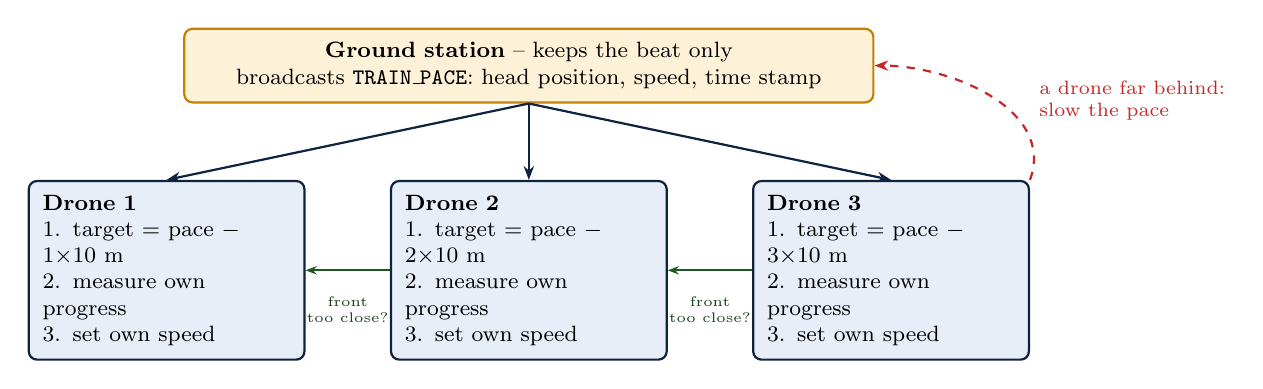
\begin{tikzpicture}[
    dbox/.style={box,text width=3.15cm,align=left,font=\footnotesize,inner sep=5pt}]
  \node[abox,text width=8.4cm,font=\footnotesize] (gcs) at (0,2.6)
    {\textbf{Ground station} -- keeps the beat only\\broadcasts \code{TRAIN\_PACE}: head position, speed, time stamp};
  \node[dbox] (d1) at (-4.6,0) {\textbf{Drone 1}\\1. target = pace $-$ 1$\times$10 m\\2. measure own progress\\3. set own speed};
  \node[dbox] (d2) at (0,0)    {\textbf{Drone 2}\\1. target = pace $-$ 2$\times$10 m\\2. measure own progress\\3. set own speed};
  \node[dbox] (d3) at (4.6,0)  {\textbf{Drone 3}\\1. target = pace $-$ 3$\times$10 m\\2. measure own progress\\3. set own speed};
  \foreach \d in {d1,d2,d3} \draw[arr] (gcs.south) -- (\d.north);
  \draw[darr,warnred] (d3.north east) to[out=70,in=0]
     node[pos=0.25,above right=1pt,font=\scriptsize,align=left,text=warnred]{a drone far behind:\\slow the pace} (gcs.east);
  \draw[-{Stealth[length=4pt]},okgreen!70!black,line width=0.8pt] (d2.west)--(d1.east);
  \draw[-{Stealth[length=4pt]},okgreen!70!black,line width=0.8pt] (d3.west)--(d2.east);
  \node[font=\tiny,text=okgreen!50!black,align=center] at ($(d1.east)!0.5!(d2.west)+(0,-0.5)$) {front\\too close?};
  \node[font=\tiny,text=okgreen!50!black,align=center] at ($(d2.east)!0.5!(d3.west)+(0,-0.5)$) {front\\too close?};
\end{tikzpicture}
\caption[On-board formation keeping]{On-board formation keeping. The ground station only sends
the pace; every drone works out its own target and sets its own speed, many times per second.}
\label{fig:pace}
\end{figure}

\section{How the Two Levels Relate}
The two levels play different roles, much like a travel plan and the driver who follows it. A
travel plan is written before the trip, assuming that the roads are open. The driver is the one
who actually sees a closed road on the way and stops to ask what to do. In the same way:
\begin{itemize}
  \item \textbf{Before flight (PDDL planning).} The flags \code{communication-ok} and
        \code{neighbor-comm-ok} say that the links are assumed to work. The plan is valid only
        under this assumption.
  \item \textbf{During flight (run-time protocol).} Heartbeats, telemetry and \code{TRAIN\_PACE}
        messages actually carry the commands and reports, and missing messages show that a link
        has really failed.
  \item \textbf{When they disagree.} If the run time observes a fault (Chapter~\ref{ch:faults}),
        the mission is held and the operator decides how to continue. The planner is not called
        again.
\end{itemize}
Figure~\ref{fig:twolevels} summarises this. The PDDL conditions do not by themselves monitor real
radio links; this is discussed as a limitation in Chapter~\ref{ch:discussion}.

\begin{figure}[!htb]
\centering
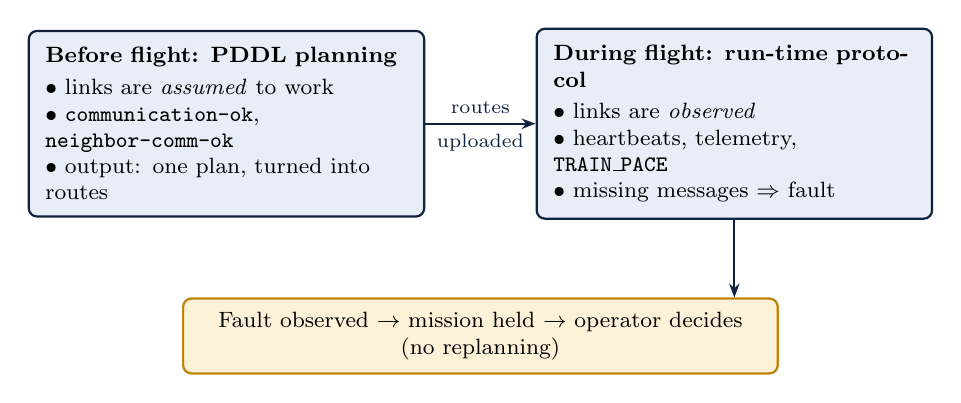
\begin{tikzpicture}[node distance=6mm and 14mm,
    col/.style={box,text width=4.6cm,align=left,font=\footnotesize,inner sep=6pt}]
  \node[col] (plan) {\textbf{Before flight: PDDL planning}\\[2pt]
     $\bullet$ links are \emph{assumed} to work\\
     $\bullet$ \code{communication-ok}, \code{neighbor-comm-ok}\\
     $\bullet$ output: one plan, turned into routes};
  \node[col,right=of plan] (run) {\textbf{During flight: run-time protocol}\\[2pt]
     $\bullet$ links are \emph{observed}\\
     $\bullet$ heartbeats, telemetry, \code{TRAIN\_PACE}\\
     $\bullet$ missing messages $\Rightarrow$ fault};
  \node[abox,below=10mm of $(plan.south)!0.5!(run.south)$,text width=7.2cm,font=\footnotesize]
     (op) {Fault observed $\rightarrow$ mission held $\rightarrow$ operator decides\\(no replanning)};
  \draw[arr] (plan.east)--node[above,font=\scriptsize]{routes}node[below,font=\scriptsize]{uploaded}(run.west);
  \draw[arr] (run.south)--(op.north -| run.south);
\end{tikzpicture}
\caption[Planning-time and run-time communication]{How planning-time and run-time communication
relate.}
\label{fig:twolevels}
\end{figure}

%% =====================================================================
%%  CHAPTER 7  FAULTS AND BATTERY HEALTH
%% =====================================================================
\chapter{Fault Modelling and Battery Health}\label{ch:faults}

\section{Faults in Simple Words}
A \emph{fault} is anything that stops a drone, or the whole swarm, from carrying out the mission
as planned. Some faults are found \emph{before} take-off, when the planner refuses to make a
plan. Others happen \emph{during} flight and are handled by the ground station and the operator.
Table~\ref{tab:simplefaults} lists the faults handled in this work, in plain words.

\begin{table}[H]
\caption{Faults handled in this work, in simple words}\label{tab:simplefaults}
\small
\begin{tabularx}{\textwidth}{@{}P{0.21\textwidth}P{0.3\textwidth}Y@{}}
\toprule
\textbf{Fault} & \textbf{What it means} & \textbf{What happens} \\
\midrule
\multicolumn{3}{@{}l}{\textit{Found before take-off (the planner refuses)}} \\
Not enough battery & The battery cannot cover a leg and still keep the return reserve. & No
plan uses that leg; if no other leg works, no plan at all. \\
No safe route & The no-fly area blocks every way from source to destination. & No plan; the
operator must change the points or the area. \\
Too many drones & The train is too long for the drawn figure-eight. & No plan; the GUI warns
before planning. \\
Wrong number of drones & For example an even number for a V, or not exactly three for a
parabola. & The request is rejected before planning. \\
Unhealthy drone & GPS, radio or health already failed before take-off. & The drone is refused
by the pre-flight check. \\
\midrule
\multicolumn{3}{@{}l}{\textit{Found during flight (the ground station reacts)}} \\
GPS lost & The drone no longer knows where it is. & The swarm is held; the operator chooses to
bring the drone back or wait for GPS. \\
Ground link lost & The drone stops hearing from, or talking to, the ground station. & Marked
degraded after a few seconds without messages, then lost. \\
Neighbour link lost & The drone can no longer talk to its formation neighbours. & The formation
cannot continue until the link is back. \\
Poor health & The drone's health score falls below the allowed minimum. & The drone leaves the
formation and the controller is told. \\
Low battery & The battery falls to the low threshold during flight. & The whole swarm is paused
and the operator decides: land now or press on. \\
Empty battery & The battery reaches zero in flight. & The drone is lost. \\
\bottomrule
\end{tabularx}
\end{table}

\section{How the Planner Models a Fault}
Every domain contains the same small family of \emph{detection} actions. Each one does three
things: it notices that a flying drone has a failed flag, it records the failure, and it takes
the drone out of the flight and out of the formation. Table~\ref{tab:faults} lists them.

\begin{table}[H]
\caption{Fault detection actions shared by the domains}\label{tab:faults}
\small
\begin{tabularx}{\textwidth}{@{}>{\ttfamily\footnotesize}P{0.29\textwidth}P{0.25\textwidth}Y@{}}
\toprule
\textbf{\normalfont\small Action} & \textbf{Fires when} & \textbf{Result} \\
\midrule
detect-gps-loss & a flying drone has no GPS & GPS marked lost; drone stops and leaves the
formation \\
detect-communication-loss & a flying drone has no ground link & link marked lost; drone stops
and leaves the formation \\
detect-neighbor-link-loss & a flying drone cannot reach its neighbours & link marked lost; drone
leaves the formation (parabola also drops all its links) \\
detect-health-failure & health falls below the minimum & health failure marked; drone stops and
leaves the formation \\
notify-ground-controller & any failure has been marked & the ground controller is informed \\
\bottomrule
\end{tabularx}
\end{table}

\noindent For example, GPS loss is detected like this:

\begin{lstlisting}
(:action detect-gps-loss
    :parameters (?d - drone)
    :precondition (and (flying ?d) (not (gps-ok ?d)))
    :effect (and (gps-lost ?d) (not (flying ?d)) (not (in-formation ?d))))
\end{lstlisting}

\noindent In words: if a drone is flying and its GPS is not OK, mark its GPS as lost, stop it and
remove it from the formation. Because every movement and formation action also needs the health
flags (\code{gps-ok}, \code{communication-ok}, \code{drone-healthy} and, in formations,
\code{neighbor-comm-ok}), a drone with a failed flag simply cannot be moved by any plan. The
planner therefore never flies an unhealthy drone, and a failed member stops the formation actions
that depend on it.

\section{What the Ground Controller Can Order}
In the point-to-point domain, once the controller has been told about a failure it can choose
one of three orders (Figure~\ref{fig:faultflow}):
\begin{itemize}
  \item \textbf{Return}: the drone flies back to the source over a safe route, if its battery
        covers the way back (\code{controller-order-return}, \code{return-to-source}).
  \item \textbf{Hover}: the drone stays where it is. Hovering uses battery, so when the battery
        reaches the return reserve the drone is switched to a return
        (\code{controller-order-hover}, \code{hover}, \code{initiate-low-battery-return}).
  \item \textbf{Sacrifice}: the drone lands immediately where it is, because it cannot be
        recovered (\code{sacrifice-drone}).
\end{itemize}

\begin{figure}[H]
\centering
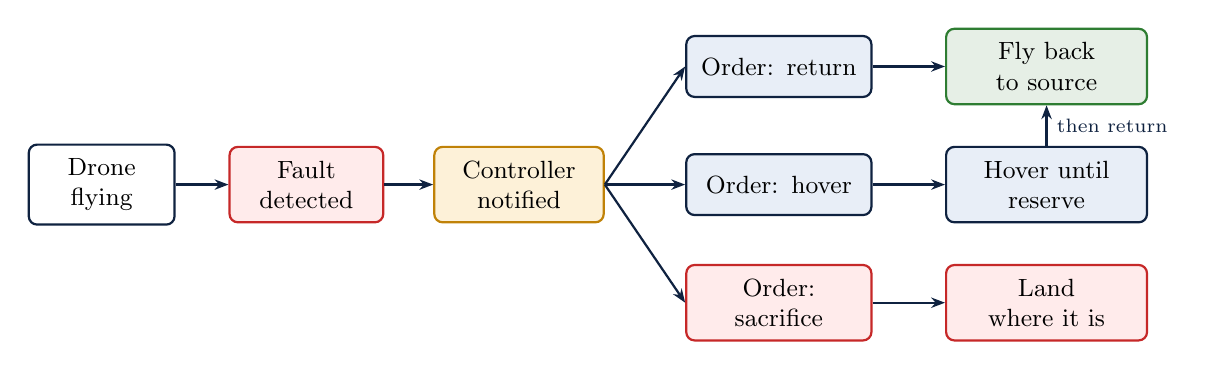
\begin{tikzpicture}[every node/.style={font=\footnotesize}]
  \node[box,fill=white,text width=1.5cm] (fl) at (0,0) {Drone\\flying};
  \node[box,fill=red!8,draw=warnred,text width=1.6cm] (det) at (2.6,0) {Fault\\detected};
  \node[abox,text width=1.8cm] (not) at (5.3,0) {Controller\\notified};
  \node[box,text width=2.0cm] (ret) at (8.6,1.5) {Order: return};
  \node[box,text width=2.0cm] (hov) at (8.6,0) {Order: hover};
  \node[box,text width=2.0cm,fill=red!8,draw=warnred] (sac) at (8.6,-1.5) {Order: sacrifice};
  \node[box,fill=okgreen!12,draw=okgreen,text width=2.2cm] (src) at (12.0,1.5) {Fly back to source};
  \node[box,text width=2.2cm] (low) at (12.0,0) {Hover until reserve};
  \node[box,text width=2.2cm,fill=red!8,draw=warnred] (land) at (12.0,-1.5) {Land where it is};
  \draw[arr] (fl)--(det); \draw[arr] (det)--(not);
  \draw[arr] (not.east)--(ret.west); \draw[arr] (not)--(hov); \draw[arr] (not.east)--(sac.west);
  \draw[arr] (ret)--(src); \draw[arr] (hov)--(low); \draw[arr] (sac)--(land);
  \draw[arr] (low)--node[right,font=\scriptsize]{then return}(src);
\end{tikzpicture}
\caption[Ground-controller responses to a fault]{Ground-controller responses in the
point-to-point domain: a detected fault is reported, and the controller orders a return, a hover
or a sacrifice.}
\label{fig:faultflow}
\end{figure}

\section{Battery as a Planning Resource}
Battery is a number in every domain, with 100 meaning a full charge. The planner uses it in three
simple ways.

\paragraph{Every leg costs energy}
Each leg has an \code{energy-required} value. When a template is retargeted, this value is
recomputed from the new leg length at the leg's own energy-per-metre rate, with a default of
0.0125 units per metre (12.5 units per kilometre). A drone may fly a leg only if its battery is
greater than the cost, and the cost is then taken away.

\paragraph{Climbing, following and hovering cost energy too}
Formation plans charge \code{climb-energy} for the climb to cruise altitude (in the parabola
plan 4 units for the vertex and 5 for the arms, which climb 10\,m further), and
\code{cruise-leg-energy} (12 units) for each follower leg. The travel domain charges
\code{hover-energy} for each hover step.

\paragraph{Always keep enough to get home}
Every drone keeps a \code{minimum-return-battery} of 30 units. The pre-flight check refuses a
drone whose battery is not above this reserve, every leg is checked as affordable or not, and the
hover and search domains switch to a return when the battery reaches the reserve. Health is a
separate score, so a drone can be refused for poor health even with a full battery.

\section{Battery Health at Run Time}
During flight each drone thread tracks its own battery. With the default settings a drone has a
5\,200\,mAh battery and draws a nominal 20\,A in flight; its percentage is computed from the
charge used. The drone classifies its own health from the battery and the GPS fix
(Figure~\ref{fig:battery}): \code{NOMINAL} above 20\,\%, \code{DEGRADED} at or below 20\,\% or
without GPS, \code{CRITICAL} at or below 5\,\%, and \code{FAILED} if the battery runs out in
flight, in which case the drone is lost.

\begin{figure}[H]
\centering
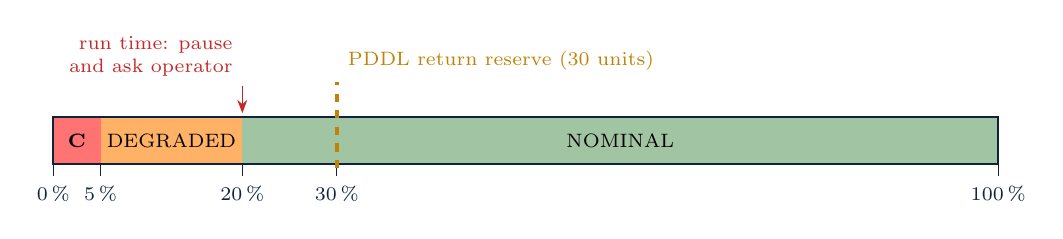
\begin{tikzpicture}
  \def\W{12}
  \fill[red!55]      (0,0) rectangle (0.05*\W,0.6);
  \fill[orange!60]   (0.05*\W,0) rectangle (0.20*\W,0.6);
  \fill[okgreen!45]  (0.20*\W,0) rectangle (\W,0.6);
  \draw[navy,line width=0.8pt] (0,0) rectangle (\W,0.6);
  \foreach \p/\l in {0/0\,\%,0.05/5\,\%,0.20/20\,\%,0.30/30\,\%,1/100\,\%}
    \draw[navy] (\p*\W,0)--(\p*\W,-0.15) node[below,font=\scriptsize]{\l};
  \node[font=\scriptsize] at (0.025*\W,0.3) {\textbf{C}};
  \node[font=\scriptsize] at (0.125*\W,0.3) {DEGRADED};
  \node[font=\scriptsize] at (0.6*\W,0.3) {NOMINAL};
  \draw[amber!80!black,line width=1.4pt,dashed] (0.30*\W,-0.05)--(0.30*\W,1.05)
     node[above right,font=\scriptsize,align=left]{PDDL return reserve (30 units)};
  \draw[-{Stealth},warnred] (0.20*\W,1.0) node[above left,font=\scriptsize,align=right,text=warnred]{run time: pause\\and ask operator}--(0.20*\W,0.65);
\end{tikzpicture}
\caption[Battery thresholds at planning time and run time]{Battery thresholds. Below the bar:
run-time health classes (C = CRITICAL; FAILED at 0\,\% in flight). The planner keeps a 30-unit
reserve; at 20\,\% the run time holds the swarm and asks the operator.}
\label{fig:battery}
\end{figure}

\noindent When any drone reaches the low-battery threshold, the ground station \emph{pauses the
whole mission} so that the drones do not drain while the operator decides; at the simulator's
compressed time scale the decision window would otherwise be a fraction of a second. A dialog
shows the drone's battery and the nearest landing point, with a note whether it is within reach
on the remaining charge. The operator may divert and land now, or press on, in which case the
drone will be lost when the battery runs flat. A drone whose battery reaches zero in flight is
reported as lost.

\section{Fault Injection and Operator Decisions}
The GUI's fault injection panel lets the operator pick one or more drones by SYSID and give them
a fault (GPS loss, communications loss or battery failure), a severity and a duration (zero
meaning until reset). In the thread-based backend, GPS loss is delivered as a \code{SET\_GPS}
command, so the drone itself loses its fix. On GPS loss the ground station holds the swarm and
asks the operator whether the drone should fall back to its start point and land, showing the
distance back and whether the remaining charge covers it; otherwise the drone holds position
until GPS returns, while its battery keeps draining. When GPS comes back the mission resumes.
Table~\ref{tab:faultmap} puts the planning side and the flight side of each fault next to each
other.

\begin{table}[H]
\caption{Each fault at planning time and during flight}\label{tab:faultmap}
\small
\begin{tabularx}{\textwidth}{@{}P{0.17\textwidth}P{0.34\textwidth}Y@{}}
\toprule
\textbf{Fault} & \textbf{In the plan (PDDL)} & \textbf{During flight} \\
\midrule
GPS loss & \code{gps-ok} false; \code{detect-gps-loss} & injected with \code{SET\_GPS}; swarm
held; operator chooses fall-back or hold \\
Ground link loss & \code{communication-ok} false; \code{detect-communication-loss} & noticed from
missing heartbeats (degraded after 5\,s, lost after 10\,s) \\
Neighbour link loss & \code{neighbor-comm-ok} false; \code{detect-neighbor-link-loss} & formation
keeping holds back (front-drone cap, slower pace) \\
Poor health & \code{health} below \code{minimum-health}; \code{detect-health-failure} & drone
health classes \code{NOMINAL}, \code{DEGRADED}, \code{CRITICAL}, \code{FAILED} \\
Low battery & battery not above the reserve; leg refused, or return started & at 20\,\% swarm
paused, operator chooses landing or press on; at 0\,\% drone lost \\
\bottomrule
\end{tabularx}
\end{table}

%% =====================================================================
%%  CHAPTER 8  RESULTS
%% =====================================================================
\chapter{Verification and Results}\label{ch:results}

\section{Method}
Each plan was verified in two ways. First, ENHSP was run directly on problems produced by the real
expand, retarget and solve pipeline, for a range of drone counts. Second, the resulting routes were
flown headless through the drone threads, and the spacing, altitudes and landing positions were
measured. Negative tests were added where a plan must refuse a problem. The run logs in
\code{plans/*/runs/} record the in-app requests.

The earlier measurements below are kept as results for the earlier plan versions. They are
not new measurements of the updated plans. Results for the changed shows and new simulator
plans are taken from the local plan status notes dated 29--30 October 2026. This report update
checks the model and source files; it does not repeat those flight experiments.

\section{In-App Planning Requests}
Table~\ref{tab:runs} summarises the logged requests for the four longest-running plans. Every
unsolvable travel and V request was traced to an infeasible combination of source, destination
and no-fly area, where no safe path existed. The grid failures all occurred in a short window
before a template fix (Section~\ref{sec:defects}); every grid request after the fix solved.

\begin{table}[H]
\caption{Logged planning requests per plan}\label{tab:runs}
\small
\begin{tabularx}{\textwidth}{@{}lrrrY@{}}
\toprule
\textbf{Plan} & \textbf{Runs} & \textbf{Solved} & \textbf{Unsolvable} & \textbf{Notes} \\
\midrule
Forest search & 69 & 69 & 0 & no failures on record \\
Travel        & 83 & 76 & 7 & infeasible no-fly inputs during early testing \\
V formation   & 65 & 62 & 2 & 2 infeasible inputs; 1 run closed mid-plan \\
Grid          & 19 & 15 & 4 & all 4 before the hover-altitude fix \\
\bottomrule
\end{tabularx}
\end{table}

\section{Scalability of the Cube Formation}
Table~\ref{tab:cube} and Figure~\ref{fig:cubeplot} show planning time and plan length for the
cube formation. Plan length grows linearly with the number of drones, about four actions per
drone. Planning time stays below 4\,s up to 36 drones and reaches 50\,s for a full $4\times4\times4$
block of 64 drones. A launch-order audit of the 25-drone plan found no drone taking off before
its layer opened and no layer opening before the one below had finished climbing.

\begin{table}[H]
\caption{Cube formation: ENHSP results through the real pipeline}\label{tab:cube}
\small
\begin{tabular*}{\textwidth}{@{\extracolsep{\fill}}lrrrrrrrr@{}}
\toprule
\textbf{Drones} & 8 & 9 & 12 & 16 & 25 & 27 & 36 & 64 \\
\textbf{Shape} & $2{\times}2{\times}2$ & $3{\times}2{\times}2$ & $2{\times}3{\times}3$ & $2{\times}3{\times}3$ &
 $3{\times}3{\times}3$ & $3{\times}3{\times}3$ & $3{\times}4{\times}4$ & $4{\times}4{\times}4$ \\
\midrule
Time (s) & 0.4 & 0.5 & 0.6 & 0.7 & 1.2 & 1.8 & 3.4 & 50.0 \\
Plan length & 42 & 47 & 58 & 74 & 111 & 119 & 155 & 268 \\
\bottomrule
\end{tabular*}
\end{table}

\begin{figure}[H]
\centering
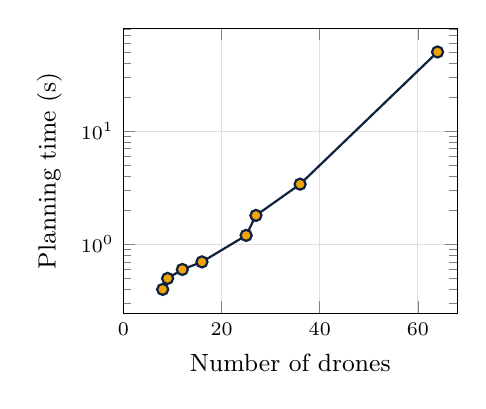
\begin{tikzpicture}
\begin{axis}[
  width=0.48\textwidth,height=5.2cm,
  xlabel={Number of drones},ylabel={Planning time (s)},
  ymode=log,log basis y=10,
  grid=major,grid style={gray!25},
  tick label style={font=\scriptsize},label style={font=\small},
  xmin=0,xmax=68,
]
\addplot[navy,thick,mark=*,mark options={fill=amber,draw=navy}] coordinates
  {(8,0.4)(9,0.5)(12,0.6)(16,0.7)(25,1.2)(27,1.8)(36,3.4)(64,50.0)};
\end{axis}
\end{tikzpicture}\hfill
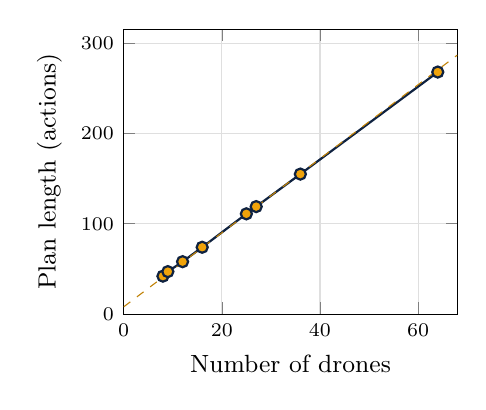
\begin{tikzpicture}
\begin{axis}[
  width=0.48\textwidth,height=5.2cm,
  xlabel={Number of drones},ylabel={Plan length (actions)},
  grid=major,grid style={gray!25},
  tick label style={font=\scriptsize},label style={font=\small},
  xmin=0,xmax=68,ymin=0,
]
\addplot[navy,thick,mark=*,mark options={fill=amber,draw=navy}] coordinates
  {(8,42)(9,47)(12,58)(16,74)(25,111)(27,119)(36,155)(64,268)};
\addplot[amber!80!black,dashed,domain=0:68] {4.1*x+8};
\end{axis}
\end{tikzpicture}
\caption[Cube formation scalability]{Cube formation scalability. Left: planning time (log scale).
Right: plan length, close to linear in the number of drones (dashed line $\approx 4.1N + 8$).}
\label{fig:cubeplot}
\end{figure}

\section{Figure-Eight Capacity and Flight Quality}
On an asymmetric eight with lobes of 337\,m and 281\,m, the computed capacity was 27 drones. ENHSP
solved every count up to 27 and returned no plan for 28, in agreement with the Python check
(Table~\ref{tab:fig8}). With a full 27-drone train, the minimum distance between any two drones at
any waypoint step was 9.85\,m, including at the crossing. Ten drones with 20 laps solved in 0.8\,s,
because laps are counted in PDDL and flown on board with a single repeat instruction rather than
being unrolled.

\begin{table}[H]
\caption{Figure-eight train: ENHSP results on an eight of capacity 27}\label{tab:fig8}
\small
\begin{tabular*}{\textwidth}{@{\extracolsep{\fill}}lrrrrrr@{}}
\toprule
\textbf{Drones} & 2 & 5 & 12 & 25 & 27 & 28 \\
\midrule
Time (s) & 0.4 & 0.4 & 0.7 & 2.7 & 3.3 & -- \\
Plan length & 26 & 38 & 66 & 118 & 126 & no plan (as intended) \\
\bottomrule
\end{tabular*}
\end{table}

\noindent After formation keeping moved on board (Section~\ref{sec:pace}), a replay of a logged
16-drone, 2-lap run changed from a median neighbour gap of 23.7\,m with a minimum of 0.0\,m
(collisions) to a median of 10.0\,m, with 90\,\% of samples between 9.2 and 10.8\,m, and every
drone landed on its own pad.

\section{Other Plans}
Table~\ref{tab:other} summarises the verification of the remaining plans.

\begin{table}[H]
\caption{Verification summary of the remaining plans}\label{tab:other}
\small
\begin{tabularx}{\textwidth}{@{}lY@{}}
\toprule
\textbf{Plan} & \textbf{Result} \\
\midrule
V formation & 3-, 5- and 7-drone V's solve through the real pipeline after the neighbour chain was
added. \\
Parabola & 27-step plan with a detour, about 0.03--0.1\,s. Negative checks (arm at 55\,m, flat
50\,m line, communication range 15\,m) give no plan. In flight, altitudes held at 50/60/60\,m,
vertex--arm gap 14.1--15.0\,m on a straight 1\,km route. \\
Star show & Updated source-to-show model: 6 drones 0.9\,s; 40 drones with 5 laps 2.3\,s.
Sampled timed tracks for 6--40 drones: closest pair 9.1\,m; all tracks end on their source pads. \\
Planets & Updated 2--8 drone model, 1--2 laps: 0.5--0.7\,s. Sampled timed tracks: about
10.0\,m minimum gap and aligned spokes. The status notes do not record a completed drone-thread
flight after this change; the attempted run received no UDP heartbeats. \\
Road inspection & 1.4\,km and 3.8\,km real roads followed with no measurable deviation from the
road line; ENHSP 0.3\,s; a source 393\,m off the road was correctly refused. \\
\bottomrule
\end{tabularx}
\end{table}

\section{Results for the New Simulator Plans}
The local status notes record the following checks. Planning results, sampled tracks and
drone-thread flight results are different checks and are reported separately.
\begin{table}[H]
\caption{Recorded checks for the new simulator plans}\label{tab:newresults}
\small
\begin{tabularx}{\textwidth}{@{}P{0.2\textwidth}Y@{}}
\toprule
\textbf{Plan} & \textbf{Recorded result} \\
\midrule
Battery-aware & Latest partial-charge example: 2.4\,km, 1000\,mAh drone; source to C1 to
destination. At C1 the charge rose from 39\,\% to 94\,\%; arrival was at 11.4\,\%, with no
ordinary low-battery prompt. An 80\,km route agreed with the independent shortest-path check. \\
Formula-4 & Recorded ENHSP checks: 0.5--0.7\,s up to 8\,km. A 500\,m flight made six swaps per
lane with a closest pair of 11.6\,m and heights of 50--60\,m. A 1\,km flight with different
drone speed limits also landed every drone on its own slot. \\
Formation-Circle & Recorded ENHSP checks: 0.4--0.5\,s up to 6\,km. Repeated 500\,m flights
measured 13.1--13.2\,m closest separation; a 1\,km flight measured 13.5\,m. Every drone landed
on its own pad. One earlier flight stalled; later successful flights do not remove that open concern. \\
\bottomrule
\end{tabularx}
\end{table}
Negative formula checks rejected unsafe gaps, excessive turning rates and an unsafe circle
height. After message splitting was added, the notes record completed 3 and 10\,km circle
flights and a 6\,km Formula-4 flight. These recorded examples do not prove safety for all inputs.
Task allocation is connected in the source code, but has no recorded successful flight result
in the checked notes, so no flight measurement is given for it.

\section{A Complete Sample Plan}\label{sec:sampleplan}
The parabola plan below, from a logged run with one detour location, shows the whole life cycle:
pre-flight checks, take-offs and climbs, six link set-ups and three confirmations, slots,
formation, two legs each followed by a shape hold, and completion.

\recordlabel{ENHSP output --- parabola formation with one detour}
\begin{lstlisting}[style=plain]
  0.0: (pre-flight-check drone-vertex source)
  1.0: (takeoff drone-vertex source)
  2.0: (climb-to-cruise-altitude drone-vertex)
  3.0: (pre-flight-check drone-left source)
  4.0: (takeoff drone-left source)
  5.0: (climb-to-cruise-altitude drone-left)
  6.0: (pre-flight-check drone-right source)
  7.0: (takeoff drone-right source)
  8.0: (climb-to-cruise-altitude drone-right)
  9.0: (establish-comm-link drone-vertex drone-right)
 10.0: (establish-comm-link drone-vertex drone-left)
 11.0: (confirm-swarm-comm drone-vertex)
 12.0: (establish-comm-link drone-left drone-vertex)
 13.0: (establish-comm-link drone-left drone-right)
 14.0: (establish-comm-link drone-right drone-left)
 15.0: (establish-comm-link drone-right drone-vertex)
 16.0: (confirm-swarm-comm drone-right)
 17.0: (confirm-swarm-comm drone-left)
 18.0: (take-parabola-slot drone-vertex)
 19.0: (take-parabola-slot drone-left)
 20.0: (take-parabola-slot drone-right)
 21.0: (establish-parabola-formation drone-vertex source)
 22.0: (formation-cruise drone-vertex source detour1)
 23.0: (hold-parabola-shape drone-vertex detour1)
 24.0: (formation-cruise drone-vertex detour1 destination)
 25.0: (hold-parabola-shape drone-vertex destination)
 26.0: (complete-parabola-mission drone-vertex destination)
Plan-Length: 27   Planning Time: 31 ms   Expanded Nodes: 28   States Evaluated: 77
\end{lstlisting}

\section{Defects Found and Fixed}\label{sec:defects}
Verification found several modelling defects. They are recorded here because each one taught a
general lesson about writing PDDL for a template-expanding pipeline.

\begin{table}[H]
\caption{Modelling defects found during verification}\label{tab:defects}
\small
\begin{tabularx}{\textwidth}{@{}P{0.2\textwidth}P{0.36\textwidth}Y@{}}
\toprule
\textbf{Plan} & \textbf{Defect} & \textbf{Fix and lesson} \\
\midrule
Grid & \code{hover-altitude} facts were written over three lines. The line-by-line cloner copied
only the middle line, leaving the value undefined for every added drone; AIBR then reported any
grid larger than $1\times2$ as unsolvable. & Rewritten as one line per fact. Templates must keep
one fact per line. \\
Cube & Layer gate written as a comparison of two fluents. A 25-drone, 3-layer cube did not solve
in 90\,s. & Replaced by propositional layer objects; solved in 1.2\,s. Prefer propositional
gates for ordering. \\
Cube & A quantified variable \code{?l} in \code{establish-cube-formation} shadowed the action's
location parameter, making every problem unsolvable. & Variable renamed. Never reuse a parameter
name inside a quantifier. \\
V formation & Readiness checked only the ground link; there was no notion of which drones sit
next to each other. & Added \code{wing-neighbor} chain and \code{neighbor-comm-ok}, with
\code{detect-neighbor-link-loss}. \\
Figure-8 & Ground-station correction caused oscillation and collisions in a 16-drone train. &
Formation keeping moved on board with a shared pace (Section~\ref{sec:pace}). \\
\bottomrule
\end{tabularx}
\end{table}

%% =====================================================================
%%  CHAPTER 9  DISCUSSION
%% =====================================================================
\chapter{Discussion and Limitations}\label{ch:discussion}

\section{What the Models Guarantee}
A plan returned by ENHSP is a proof, within the model, that the mission can be completed without
breaking any of the written rules: no drone flies with a failed flag, no move exceeds the battery,
no formation forms without all its members in contact, the cube never climbs a layer through
another, and the figure-eight never carries more drones than it can hold. Because these rules are
written in readable PDDL, they can be reviewed directly, and a change to a rule takes effect in
every mission that uses it.

\section{Limitations}
The present work has the following limitations, in simple terms.
\begin{itemize}[itemsep=5pt]
  \item \textbf{Height and terrain have limits.} Formula-4 and Formation-Circle change height
        during flight. A separate route helper also samples artificial hills and can raise a
        route or add a bypass. This is computed terrain, not measured ground data. It does not
        prove that every formation member clears real hills or buildings.

  \item \textbf{No replanning when a plan fails.} The symbolic plan is made before take-off. Task allocation can replace a failed owner
        through its runtime controller, but that controller does not run ENHSP again. If a
        drone fails or the route becomes blocked during the flight, the planner is not called
        again: the swarm is paused and the operator decides what to do.
  \item \textbf{No backup plans.} The fault detection actions record a failure, but the planner
        never prepares a ``plan B'' in advance, such as which drone should take over a lost
        drone's place.
  \item \textbf{Communication is assumed, not measured.} The PDDL flags say that the links are
        expected to work. They are not updated from real radio signal strength during the
        flight.
  \item \textbf{Battery in model units.} Most earlier plans use a 0--100 scale, not real
        milliampere-hours. The planning reserve and the run-time low-battery threshold are
        therefore separate safeguards in those plans. Battery-aware travel instead estimates
        each hop from the simulated current draw and battery capacity, with a 10\,\% margin.
        This still needs calibration before use on physical drones.
  \item \textbf{Only fixed, known no-fly areas.} One restricted area is drawn before planning.
        Moving obstacles, other aircraft, wind and weather are not modelled.
  \item \textbf{Followers are not checked one by one.} Only the leader's path is planned. The
        followers' paths are derived from it by fixed offsets, with a wider safety margin
        around the no-fly area, so the planner does not check each follower's path on its own.
  \item \textbf{Planning time grows for some formations.} The V formation becomes slow to plan as
        the swarm grows: beyond \maxV{} drones it no longer finishes within the simulator's
        planning time limit, while the grid and the cube scale much further.
  \item \textbf{Partial fault injection.} The GUI offers GPS loss, communications loss and battery
        failure, but in the thread-based backend only GPS loss is currently delivered to the
        drones.
  \item \textbf{Simulation only.} All results come from the simulator. No physical flight was
        performed, and the road inspection plan depends on an external routing service.
\end{itemize}

%% =====================================================================
%%  CHAPTER 10  CONCLUSION
%% =====================================================================
\chapter{Conclusion and Future Work}\label{ch:conclusion}

\section{Conclusion}
This thesis presented the PDDL planning layer of a drone swarm simulator. Fourteen simulator
mission plans cover travel, area search, rigid formations, a figure-eight train, two shows,
road inspection, battery-aware travel and two moving four-drone formations. The swarm templates
adapt to selected counts within their limits; the new formula formations use four drones and
battery-aware travel uses one. Task allocation adds a PDDL ownership model and a runtime controller that launches a standby
and relays mission data after a fault. Its runtime handling is separate from symbolic replanning. Communication was modelled as neighbour relations with
per-drone flags, and, in the parabola plan, as an explicit mesh of range-checked links. Faults
were modelled as detection actions with ground-controller responses, and battery as a numeric
resource with a return reserve, complemented at run time by thresholds that pause the swarm and
ask the operator.

The plans run through the real pipeline: they are retargeted to map inputs, expanded to the
selected number of drones, solved by ENHSP and flown by the drone threads. The results show that
careful modelling keeps planning fast for realistic swarm sizes: 64 drones in a cube in 50\,s,
a 27-drone figure-eight train in 3.3\,s, and most missions in well under a second. The defects
found during verification led to general modelling rules that will help anyone extending the
plans.

\section{Future Work}
\begin{enumerate}[itemsep=5pt]
  \item \textbf{Verify task allocation end to end.} Test repeated handoffs, failed replacements,
        missing radio messages and cases where no healthy standby remains. Check that the
        runtime state follows the PDDL ownership rules.
  \item \textbf{Online replanning.} Feed run-time faults back into the PDDL state and replan the
        remaining mission, for example closing a formation around a lost drone.
  \item \textbf{Calibrated energy model.} Derive \code{energy-required} and the reserve from the
        drone's battery capacity, current draw, speed and wind, so that planning and run-time
        thresholds use the same units.
  \item \textbf{A local planner on every drone.} Give each drone its own small on-board planner,
        so that it can make quick local decisions by itself -- for example moving around a
        sudden obstacle or closing the gap when a neighbour is lost -- without waiting for the
        ground station. The PDDL plan from the ground would still set the overall mission, while
        each drone's local planner handles what happens around it.
  \item \textbf{Complete fault injection.} Deliver communication loss and battery failure faults
        to the drone threads, matching the GUI options, and test the operator responses under
        each.
  \item \textbf{Larger formations.} Reduce planning cost for formations that grow slowly, such as
        the V, for example by the same propositional restructuring that made the cube scale.
  \item \textbf{Tests on real drones.} Fly the plans with hardware in the loop and, eventually,
        on physical drones.
\end{enumerate}

%% =====================================================================
%%  REFERENCES
%% =====================================================================
\clearpage
\phantomsection
\addcontentsline{toc}{chapter}{References}
\renewcommand{\bibname}{References}
\begin{thebibliography}{99}
\setlength{\itemsep}{3pt}
\bibitem{mcdermott1998pddl} D. McDermott, M. Ghallab, A. Howe, C. Knoblock, A. Ram, M. Veloso,
  D. Weld and D. Wilkins, \emph{PDDL -- The Planning Domain Definition Language}, Technical Report
  CVC TR-98-003, Yale Center for Computational Vision and Control, 1998.
\bibitem{fox2003pddl21} M. Fox and D. Long, \emph{PDDL2.1: An Extension to PDDL for Expressing
  Temporal Planning Domains}, Journal of Artificial Intelligence Research, vol.~20, pp.~61--124,
  2003.
\bibitem{ghallab2004automated} M. Ghallab, D. Nau and P. Traverso, \emph{Automated Planning:
  Theory and Practice}, Morgan Kaufmann, 2004.
\bibitem{scala2016interval} E. Scala, P. Haslum, S. Thi\'ebaux and M. Ramirez,
  \emph{Interval-Based Relaxation for General Numeric Planning}, Proceedings of the 22nd European
  Conference on Artificial Intelligence (ECAI), pp.~655--663, 2016.
\bibitem{scala2020subgoaling} E. Scala, P. Haslum, S. Thi\'ebaux and M. Ramirez,
  \emph{Subgoaling Techniques for Satisficing and Optimal Numeric Planning}, Journal of Artificial
  Intelligence Research, vol.~68, pp.~691--752, 2020.
\bibitem{chung2018survey} S.-J. Chung, A. A. Paranjape, P. Dames, S. Shen and V. Kumar,
  \emph{A Survey on Aerial Swarm Robotics}, IEEE Transactions on Robotics, vol.~34, no.~4,
  pp.~837--855, 2018.
\bibitem{brambilla2013swarm} M. Brambilla, E. Ferrante, M. Birattari and M. Dorigo,
  \emph{Swarm Robotics: A Review from the Swarm Engineering Perspective}, Swarm Intelligence,
  vol.~7, no.~1, pp.~1--41, 2013.
\bibitem{reynolds1987flocks} C. W. Reynolds, \emph{Flocks, Herds and Schools: A Distributed
  Behavioral Model}, Proceedings of SIGGRAPH '87, Computer Graphics, vol.~21, no.~4, pp.~25--34,
  1987.
\bibitem{dubins1957curves} L. E. Dubins, \emph{On Curves of Minimal Length with a Constraint on
  Average Curvature, and with Prescribed Initial and Terminal Positions and Tangents}, American
  Journal of Mathematics, vol.~79, no.~3, pp.~497--516, 1957.
\bibitem{luxen2011osrm} D. Luxen and C. Vetter, \emph{Real-Time Routing with OpenStreetMap Data},
  Proceedings of the 19th ACM SIGSPATIAL International Conference on Advances in Geographic
  Information Systems, pp.~513--516, 2011.
\bibitem{mavlink} MAVLink Development Team, \emph{MAVLink Micro Air Vehicle Communication
  Protocol}, \url{https://mavlink.io/en/}.
\bibitem{enhsp} E. Scala, \emph{ENHSP -- Expressive Numeric Heuristic Search Planner},
  \url{https://sites.google.com/view/enhsp/}.
\bibitem{pyside6} The Qt Company, \emph{Qt for Python (PySide6)},
  \url{https://doc.qt.io/qtforpython-6/}.
\end{thebibliography}

\end{document}
